\documentclass[11pt]{article}

\usepackage{times}
%\usepackage[hidelinks]{hyperref}
\usepackage{hyperref}
\usepackage{enumerate}
\usepackage[letterpaper, margin=0.75in]{geometry}
\usepackage{amsmath}
%\usepackage{pdfpages}
\usepackage{graphicx,subfigure}
%\graphicspath{{figures/}}
%\usepackage[font={small},skip=-3pt]{caption}
\usepackage[font=small]{caption}
%\captionsetup[figure]{font=small,skip=0pt}
\renewcommand{\topfraction}{0.85}
\renewcommand{\textfraction}{0.1}
\renewcommand{\floatpagefraction}{0.85}
\usepackage{color}
\usepackage[section]{placeins}
\usepackage{authblk}

\usepackage{xcolor}
\hypersetup{
    colorlinks,
    linkcolor={red!50!black},
    citecolor={blue!50!black},
    urlcolor={blue!80!black}
}

\renewcommand\Authands{ and }

\title{Expanded View}
\author[1,2,*]{Aaron N. Brooks}
\author[1,*,$\dag$]{David J. Reiss}
\author[3]{Antoine Allard}
\author[1]{Wei-Ju Wu}
\author[4]{Diego M. Salvanha}
\author[1]{Christopher L. Plaisier}
\author[1]{Sriram Chandrasekaran}
\author[1]{Min Pan}
\author[1]{Amardeep Kaur}
\author[1,2,5,6,$\dag$]{Nitin S. Baliga}
\affil[1]{Institute for Systems Biology, 1441 N 34th Street, Seattle, WA 98103}
\affil[2]{Molecular and Cellular Biology Program, University of Washington, Seattle, WA 98195}
\affil[3]{Département de Physique, de Génie Physique et d'Optique, Université Laval, Québec, QC, Canada}
\affil[4]{LabPIB, Department of Computing and Mathematics FFCLRP-USP, University of Sao Paulo, Ribeirao Preto, Brazil}
\affil[5]{Departments of Microbiology and Biology, University of Washington, Seattle, WA 98195}
\affil[6]{Lawrence Berkeley National Laboratories, Berkeley, CA 94720}
\affil[*]{Equal contribution}
\affil[$\dag$]{To whom correspondence should be addressed: \newline \href{mailto:nbaliga@systemsbiology.org}{nbaliga@systemsbiology.org}; \href{mailto:dreiss@systemsbiology.org}{dreiss@systemsbiology.org}}
\date{\today}

%%%%%%%%%% This allows ``paragraph'' to be  like a subsubsubsection
%%%%%%%%%% from here https://tex.stackexchange.com/questions/60209/how-to-add-an-extra-level-of-sections-with-headings-below-subsubsection
\makeatletter
\renewcommand\paragraph{\@startsection{paragraph}{4}{\z@}%
            {-2.5ex\@plus -1ex \@minus -.25ex}%
            {1.25ex \@plus .25ex}%
            {\normalfont\small\bfseries}}
\makeatother
\setcounter{secnumdepth}{4} % how many sectioning levels to assign numbers to
\setcounter{tocdepth}{4}    % how many sectioning levels to show in ToC

%%%%%%%%%% This adds 'E' to figure name for expanded view
\makeatletter 
\renewcommand{\thefigure}{E\@arabic\c@figure}
\makeatother

%%%%%%%%%% Start TeXmacs macros
\newcommand{\email}[1]{{\textit{Email:} \texttt{#1}}}
\newcommand{\tmem}[1]{{\em #1\/}}
\newcommand{\tmhlink}[2]{{\color{blue} #1}}
\newcommand{\tmmathbf}[1]{\ensuremath{\boldsymbol{#1}}}
\newcommand{\tmname}[1]{\textsc{#1}}
\newcommand{\tmop}[1]{\ensuremath{\operatorname{#1}}}
\newcommand{\tmsamp}[1]{\textsf{#1}}
\newcommand{\tmtextit}[1]{{\itshape{#1}}}
\newenvironment{enumeratenumeric}{\begin{enumerate}[1.] }{\end{enumerate}}
\newcommand{\tmfloatcontents}{}
\newlength{\tmfloatwidth}
\newcommand{\tmfloat}[5]{
  \renewcommand{\tmfloatcontents}{#4}
  \setlength{\tmfloatwidth}{\widthof{\tmfloatcontents}+1in}
  \ifthenelse{\equal{#2}{small}}
    {\ifthenelse{\lengthtest{\tmfloatwidth > \linewidth}}
      {\setlength{\tmfloatwidth}{\linewidth}}{}}
    {\setlength{\tmfloatwidth}{\linewidth}}
  \begin{minipage}[#1]{\tmfloatwidth}
    \begin{center}
      \tmfloatcontents
      \captionof{#3}{#5}
    \end{center}
  \end{minipage}}
%%%%%%%%%% End TeXmacs macros

\newcommand{\eg}{\tmtextit{e.g.}}
\newcommand{\ie}{\tmtextit{i.e.}}
\newcommand{\cm}{{\tmsamp{cMonkey}}}
\newcommand{\nwinf}{{\tmsamp{Inferelator}}}
\newcommand{\MEME}{{\tmsamp{MEME}}}
\newcommand{\halo}{{\tmem{H. salinarium NRC-1}}}
\newcommand{\eco}{{\tmem{E. coli K-12 MG1655}}}
\newcommand{\tab}{{\hspace{5mm}}}
\newcommand{\rdb}{{\tmsamp{RegulonDB}}}
\newcommand{\egrine}{{\tmsamp{EGRIN 2.0}}}
\newcommand{\simgt}{\,\hbox{\lower0.6ex\hbox{$\sim$}\llap{\raise0.6ex\hbox{$>$}}}\,}
\newcommand{\simlt}{\,\hbox{\lower0.6ex\hbox{$\sim$}\llap{\raise0.6ex\hbox{$<$}}}\,}
\newcommand{\citep}[1]{({\cite{#1}})}
\newcounter{suppfigure}

\begin{document}
\maketitle
 
\tableofcontents
\newpage
\listoffigures
\newpage
\listoftables 
\newpage

\begin{abstract}
Microbes can tailor transcriptional responses to diverse environmental
challenges despite having streamlined genomes and a limited number of
regulators. Here, we present data-driven models that capture the
dynamic interplay of the environment and genome-encoded regulatory
programs of two types of prokaryotes: E. coli (a bacterium) and
H. salinarum (an archaeon). The models reveal how the genome-wide
distributions of cis-acting gene regulatory elements and the
conditional influences of transcription factors at each of those
elements encode programs for eliciting a wide array of
environment-specific responses. We demonstrate how these programs
partition transcriptional regulation of genes within regulons and
operons to re-organize gene-gene functional associations in each
environment. The models capture fitness-relevant co-regulation by
different transcriptional control mechanisms acting across the entire
genome, to define a generalized, system-level organizing principle for
prokaryotic gene regulatory networks that goes well beyond existing
paradigms of gene regulation.
\end{abstract}

\section{Online materials}
Additional figures, tables, supporting data, and comprehensive model
predictions are available at: \newline
\url{http://egrin2.systemsbiology.net}.

\section{Experimental data used for model construction}\label{data}

\subsection{mRNA expression data}


\subsubsection{\halo~ compendium}\label{halodata}

A compendium of 1495 transcriptome profiles were collated from a wide
array of experiments conducted by our lab over the past decade that
cover dynamic transcriptional responses to varied growth (1159
arrays), nutritional (161 arrays), and stress conditions (1102
arrays), including variation in temperature (256 arrays), oxygen (285
arrays), light (786 arrays), salinity (20 arrays), metal ions (274
arrays), and genetic perturbations (643 arrays).  We categorized the
experiments using extensive metadata collected at the time of the
experiment. We used this metadata to construct a GO-like ontology of
the relationships between all experiments (discussed in detail below).
The annotation counts above are derived from this resource (note that
a single array can receive more than one annotation).  A full list of
the metadata, annotations, and ontology is available on the web
service.  1159 of the arrays are published
(\cite{Baliga2004a,Baliga2002,Bonneau2007,Facciotti2010,Facciotti2007a,Kaur2006,Kaur2010,Schmid2011,Schmid2007,Schmid2009,Whitehead2006,Whitehead2009}. 336
of the arrays are new for this study. Experimental protocols are
identical to \cite{Bonneau2007}. These data, including expression
levels (log$_2$ ratios vs. reference samples) and experimental
metadata, are available online as a tab-delimited spreadsheet.

%\paragraph{Data normalization} %% note this probably doesnt need to be a separate section

Each array in the {\it H. salinarum} compendium was collected using
the same platform, using the same reference, and processed and
normalized using the same protocol. More specifically, each RNA sample
was hybridized along with a {\it H. salinarum NRC-1} reference RNA
prepared under standard conditions (mid-logarithmic phase batch
cultures grown at 37$^{\circ}$C in CM, OD = 0.5). Samples were hybridized to a
70-mer oligonucleotide array containing the 2400 non-redundant open
reading frames (ORFs) of the {\it H. salinarum NRC-1} genome as
described in \cite{Baliga2004a}. Each ORF was spotted on each array
in quadruplicate and dye flipping was conducted (to rule out bias in
dye incorporation) for all samples, yielding eight technical
replicates per gene per sample. At least two independent biological
replicates exist for all experimental conditions for a total of 16
replicates per gene per condition. Direct RNA labeling, slide
hybridization, and washing protocols were performed as described by
\cite{Facciotti2007,Schmid2007}. Raw intensity signals
from each slide were processed by the SBEAMS-microarray pipeline
\cite{Marzolf2006a} (www.SBEAMS.org/microarray), in which the
data were median normalized and subjected to significant analysis of
microarrays (SAM) and variability and error estimates analysis
(VERA). Each data point was assigned a significance statistic,
$\lambda$, using maximum likelihood \cite{Ideker2000}.

\subsubsection{\eco~ expression compendia}\label{ecodata}

\paragraph{Use of the \tmsamp{DISTILLER} data compendium for model training}

A total of 868 \eco\ transcriptome profiles were compiled by
\cite{Lemmens2009a} for use with their \tmsamp{DISTILLER} algorithm. 
These data were collated from publicly available microarray databases:
44 arrays from Stanford Microarray Database \cite{Demeter2007d},
617 from Gene Expression Omnibus \cite{Barrett2007} and 36 from
ArrayExpress \cite{Parkinson2007}, as well as 181 arrays from
supplementary data in literature (for four different experiments). The
experiments cover a range of conditions, including varying carbon
sources (136 arrays), pH (46 arrays), oxygen (284 arrays), metals (27
arrays) and temperature (23 arrays). Overall, the compendium consists
of measurements from single channel (407 arrays; including 298 Affymetrix, 
and 109 P33) and dual channel (460 arrays; including 337 DNA/cDNA
and 126 oligonucleotide) platforms.

%\paragraph{Data normalization}

These microarray measurements were normalized by the
authors \cite{Lemmens2009a}, as follows: ``If possible, raw
intensities were preferred as data source over normalized data
provided by the public repository. Dual-channel data were loess fitted
to remove nonlinear, dye-related discrepancies. No background
correction procedures were performed to avoid an increase in
expression logratio variance for lower, less reliable intensity
levels. Whenever raw data were available, single-channel data were
first normalized per experiment with RMA. Logratios were then
created for the single-channel data in order to combine them with the
dual channel measurements. For each single-channel array, expression
logratios were computed by comparing the normalized values against an
artificial reference array.  This artificial reference array was
constructed on a per experiment basis by taking the median expression
of each gene across all arrays in the corresponding experiment. When
deemed necessary (e.g. experiments normalized by MAS5.0 for which the
raw data was not available), a loess fit was performed on these
logratios. To ensure that the artificial reference was not altered by
this intensity dependent non-linear rescaling, the artificial
reference expression levels were chosen for the average log intensity
(instead of the mean expression levels of the respective array and the
artificial reference). To ensure comparability between arrays with a
different reference, gene expression profiles were median centered
across arrays that share the same reference. An additional variance
rescaling of the gene expression profiles was performed to render
genes with differing magnitudes of expression changes more
comparable.''

The authors further note that, ``the array composition of the modules
generated by \tmsamp{DISTILLER} is not biased towards arrays from any
specific platform, indicating a correct preprocessing of the
microarray compendium.'' \cite{Lemmens2009a} It is for this reason
that we chose this normalized {\it E. coli} microarray compendium
for \egrine~analysis.

\paragraph{Use of the \tmsamp{DREAM5} data compendium for model validation}
\label{section:dream5_data_compendium}

To ascertain the generalizability of \egrine~models across data sets,
we inferred a second \textit{E. coli} \egrine~model on an
independent \textit{E. coli} gene expression compendium. By comparing
this model to the original model we inferred using
the \tmsamp{DISTILLER} data set, we were able (1) to understand what,
if any, systematic biases exist due to normalization procedures, and
(2) to cross-validate \egrine~predictions across two data
set. Detailed discussion of the results from this analysis are
provided in Section~\ref{sec:validation}.

We obtained the de-anonymized {\it E. coli} microarray compendium from
the \tmsamp{DREAM5} competition website \cite{Marbach2012}. According
to the authors, these data were ``compiled for {\it E. coli}, where
all chips are the same Affymetrix platform, the \textit{E. coli}
Antisense Genome Array. Chips were downloaded from GEO (Platform ID:
GPL199). In total, 805 chips with available raw data Affymetrix files
(.CEL files) were compiled.''  Additionally, ``Microarray
normalization was done using Robust Multichip Averaging (RMA) 9
through the software RMAExpress. All 160 chips were uploaded into
RMAExpress and normalization was done as one batch. All arrays were
background adjusted, quantile normalized, and probesets were
summarized using median polish. Normalized data was exported as
log-transformed expression values. Mapping of Affymetrix probeset ids
to gene ids was done using the library files made available from
Affymetrix. Control probesets and probesets that did not map
unambiguously to one gene were removed, specifically probeset ids
ending in \_x, \_s, \_i were removed. Lastly, if multiple probesets
mapped to a single gene, then expression values were averaged within
each chip.''

Compared to the \tmsamp{DISTILLER} \cite{Lemmens2009a} data set,
the \tmsamp{DREAM5} \cite{Marbach2012} compendium contained a
different subset of the available \textit{E. coli} transcriptome
measurements from a different combination of platforms. While one
might expect a number of arrays to be common between the two
compendia, we discovered that the two data sets differed substantially
in their statistical properties. The maximum Pearson correlation
between arrays across the two data sets, for example, was $\sim 0.63$.
Interestingly, the correlation among expression profiles of genes
within predicted operons \cite{Price2005a} was higher in the
\tmsamp{DREAM5} compendium (mean $\sim 0.83$) than the \tmsamp{DISTILLER} compendium
(mean $\sim 0.32$). This is likely due to a combination of differences
in the experiments/platforms included and normalization procedures.


\subsection{Additional data integrated for model construction}

\subsubsection{Genome sequence data and annotatations for \cm~analysis}

We used genome sequences and gene annotations (coding regions)
collated in \tmsamp{RSA-tools} \cite{vanHelden2000} for both
organisms in this study (\halo~and \eco). These data were themselves
collated to annotate regulatory sequences of all sequenced genomes in
\tmsamp{RefSeq}. Rather than using the \tmsamp{RSA-tools}-annotated
promoter regions, we computed them ourselves as regions (-250 nt to
+50 nt) surrounding the annotated translation start site of each
gene/operon (see below for operon annotations). 

In all cases where probe identifiers in the mRNA expression compendia
used for this analysis could not be directly matched to gene
annotations (or operon predictions or functional associations; see
below), we used the \tmsamp{RSA-tools} ``\tmsamp{feature\_names.tab}''
table of identifier synonyms to perform the match. In cases where the
match was still not possible, we excluded the probe/ annotation/
association from analysis.

\subsubsection{Operon membership predictions used for \cm~analysis}

We used operon predictions for both \halo~and \eco~predicted by
\cite{Price2005a} from the \tmsamp{Microbes Online}
database \cite{Alm2005}. These predictions are updated regularly. The predictions are based upon
genomic proximity and co-expression in publicly-available microarray
data compendia. We used the versions downloaded
from the website as of March, 2009. These included
predicted operon memberships for 826 genes in \halo~ and for 2,639
genes in \eco.

\subsubsection{Predicted transcriptional regulators used for \nwinf~analysis}

\paragraph{\halo}

For \halo, we used the same set of putative transcription factors
(TFs) as \cite{Bonneau2006,Bonneau2007}. This list of 124
regulators was selected from among the 2,400 \halo\ genes which are
annotated as known or putative TFs based upon sequence or predicted
structural homology \cite{Bonneau2004}.

\paragraph{\eco}
\label{section:eco_tfs}

To enable direct comparison of our results to DREAM5, we used the list
of 296 putative \eco~ transcriptional regulators collated
by \cite{Marbach2012}. Their list was obtained by combining the list
of TFs defined by RegulonDB \cite{Gama-Castro2011} with TFs identified
using Gene Ontology (GO) terms: \textit{biological process} terms
related to transcription (\texttt{GO:0009299;mRNA transcription}
or \texttt{GO:0006351;transcription, DNA dependent}) and
GO \textit{molecular function}
\texttt{GO:0003677;DNA binding} or any child terms.

\subsubsection{Functional association networks integrated into \cm~analysis}

We used EMBL STRING \cite{Szklarczyk2011} v9.0 database
of predicted functional associations between genes for both organisms
(\halo~and \eco) to constrain module construction in \cm, as described
below. The confidence scores estimated by \cite{Szklarczyk2011} were
incorporated into the \cm~constraints. These
networks included 151,826 associations among 2,559 genes in \halo, and
878,972 associations among 4,136 genes in \eco.



\section{Independent data used for model validation}


\textcolor{red}{\tmem{\textbf{Model validation data was not used for model construction. }}}

\subsection{\halo}\label{halodata}

\subsubsection{Tiling array transcriptome measurements}

We generated {\it H. salinarum NRC-1} high-resolution (12 nt) tiling
array transcriptome measurements over 12 points along the growth curve
in rich media. These were analyzed and published in a separate study
\cite{Koide2009}. Locations of putative transcription breaks in these data were
identified in \cite{Koide2009} using multivariate recursive
partitioning, including signals from both relative changes in
expression along the growth curve, as well as raw RNA hybridization
signal. For more details, see \cite{Koide2009}.

\subsubsection{ChIP-chip transcription factor binding measurements for global regulators}

Global binding of eight general transcription factors (seven TFBs
[TFBa, TFBb, TFBc, TFBd, TFBe, TFBf, and TFBg] and one TBP [TbpB]) and
three specific TFs (Trh3, Trh4, and VNG1451C) in {\it H. salinarum}
were collected in our lab by ChIP-chip. A detailed protocol is
described in \cite{Facciotti2007}. Briefly, ChIP-enriched and
amplified DNA for eleven regulators was hybridized to a low-resolution
(500~nt resolution) custom PCR-product array spotted in-house. The
resulting intensities were analyzed using
{\tmsamp{MeDiChI}} \cite{Reiss2008} to obtain binding site locations
with an average precision of 50~nt. Local false discovery rates
(LFDRs) were quantified by simulation. For more details on the
ChIP-chip analysis methodology used in this work,
see \cite{Reiss2008}.

\subsubsection{\textit{kdp} promoter serial truncation measurements}

{\it H. salinarum NRC-1} \textit{kdpFABC} truncation data were
obtained from \cite{Kixmueller2011}. Briefly, the authors measured
relative induction of a transcriptional reporter after serial
truncation of the \textit{H. salinarum} R1 \textit{kdpFABC}
promoter. The authors measured $\beta$-Galactosidase activities from
truncated transcriptional fusions of the \textit{kdpFABC} promoter
to \textit{bgaH}. $\beta$-Galactosidase activities were measured in
triplicate from cultures grown in inducing (3 mM K$^{+}$) and
non-inducing (100 mM K$^{+}$) conditions. We obtained data
corresponding to Figure~4 of the paper, in which the authors quantify
the fractional $\beta$-Galactosidase activity (non-induced/induced)
among the serial truncations (private communication). We overlaid
motif predictions from \egrine~on this data set to reach our
conclusions.

\subsection{\eco}\label{ecodata}

\subsubsection{Tiling array transcriptome measurements}
\label{section:ecoarray}

We measured \eco\ tiling array transcriptome profiles at nine
different time points during growth in rich media (LB). Growth phases
spanned lag-phase (OD600 = 0.05) to late stationary-phase (OD600 =
7.3). RNA samples were prepared by hot phenol-chloroform
extraction \cite{Khodursky2003}. RNA was directly labeled and
hybridized to custom Agilent tiling arrays containing 60mer probes
tiled across both strands of the \eco\ genome using a sliding window
of 23~nt (GEO Platform GPL18392), as in \cite{Koide2009}. Expression
measurements were quantile-normalized as in \cite{Yoon2011} and
analyzed for condition-specific transcriptional isoforms following the
segmentation protocol described in \cite{Koide2009}. Data is available
on GEO (GSE55879).

\subsubsection{PurR/$\Delta$PurR expression data and ChIP-chip transcription factor binding sites} 

{\it E. coli} PurR/$\Delta$PurR expression data and ChIP-chip
transcription factor binding measurements collected in the presence of
adenine were taken from \cite{Cho2011a}. ChIP-chip relative
intensities were re-analyzed using
{\tmsamp{MeDiChI}} \cite{Reiss2008} to obtain binding site locations
with an average precision of $\sim$25~nt.

\subsubsection{Fitness measurements}
\label{section:fitness}

{\it E. coli} fitness measurements across 324 conditions were
generated by \cite{Nichols2011}. In short, the authors quantitated
growth rates for 3979 single gene deletions in each of 324
environments with variable stress, drug, and environmental
challenges. \textit{E. coli} mutant colony sizes were quantified on
agar plates.  Fitness correlations were obtained directly from the
authors: \href{http://ecoliwiki.net/tools/chemgen/}{http://ecoliwiki.net/tools/chemgen/}. Each
correlation value represents the Pearson correlation of fitness (\ie,
relative growth rate) for pairs of single gene deletion mutants
measured across all 324 conditions that are also present in our
analysis. Relative fitness scores were also obtained directly from the
authors.

\subsubsection{Effector molecule measurements}

{\it E. coli} effector molecule measurements were taken
from \cite{Ishii2007}. The authors measured metabolite levels using
capillary electrophoresis time-of-flight mass spectrometry (CE-TOFMS)
in \eco, as well as several other biomolecules (\eg., RNA and
protein). \textit{E. coli} was grown in a chemostat at several
different dilution rates (0.1, 0.2, 0.4, 0.5, and 0.7
hours$^{–1}$). We obtained the metabolite levels from the authors and
computed Pearson correlation between metabolites assigned to regulate
TFs by RegPrecise \cite{Novichkov2010}.

\subsubsection{Experimentally mapped {\it E. coli} transcription factor binding sites}

We compared genome-wide locations of GREs in the {\it E. coli} EGRIN
2.0 model with experimentally-mapped binding sites from the \rdb
database \cite{Gama-Castro2011}. To maintain consistency with our
comparisons against the DREAM5 community networks \cite{Marbach2012},
we used version 6.8 of the database. For binding sites, we used the
{\tmsamp{BindingSiteSet}} table, filtered for only interactions with
experimental evidence, and used only TFs with $\geq 3$ unique binding
sites -- a total of 88 TFs.

\subsubsection{Experimentally measured {\it E. coli} transcription factor regulatory targets}
\label{section:eco:gold:standard}

For the {\it E. coli} gold standard network, we used the same network
as that used by \cite{Marbach2012} for validation of the DREAM5 {\it
E. coli} community predicted regulatory networks. This gold standard
is based upon version 6.8 of the \rdb~
database \cite{Gama-Castro2011}, and only interactions with at least
one strong evidence were included, for a total of 2,066 interactions.
We mapped the $aaaX$-style gene names in the DREAM5 gold standard to
the $b1234$ in \cm~using a translation table compiled in the
{\tmsamp{EcoGene}} database, version 3.0 \cite{Zhou2013a}. We were
able to map a total of 4,273 gene names. The final gold standard
consisted of 2,064 interactions between 141 TFs and 997 target
genes. The final, complete gold standard network used for all analyses
is available \href{http://egrin2.systemsbiology.net/}{online}.
%at \ref{tables:DREAM5_gold_network.tsv}.


\section{Computational methods}

\subsection{\DIFdelbegin \DIFdel{cMonkey}\DIFdelend \DIFaddbegin \cm\DIFaddend : integrated biclustering algorithm, updated for ensemble analysis}

\subsubsection{Introduction and summary}

The \cm\ integrated biclustering algorithm was described and \DIFdelbegin \DIFdel{benchmarked in (Reiss et al. , 2006). }\DIFdelend \DIFaddbegin \DIFadd{fully
benchmarked in \mbox{%DIFAUXCMD
\cite{Reiss2006n}
}%DIFAUXCMD
. }\DIFaddend In short, the algorithm computes
putatively co-regulated modules of genes over subsets of experimental
conditions from gene expression data, constrained by information
provided by genome sequence (\DIFdelbegin \DIFdel{in the form of de novo }\DIFdelend \DIFaddbegin \textit{\DIFadd{de novo}} \DIFaddend identification of
conserved \DIFdelbegin \DIFdel{cis-regulatory motifs in the }\DIFdelend \DIFaddbegin \textit{\DIFadd{cis}}\DIFadd{-regulatory motifs in }\DIFaddend gene promoters), and functional
association networks. Its defining characteristic is that it
\DIFdelbegin \DIFdel{integrates }\DIFdelend \DIFaddbegin \DIFadd{combines }\DIFaddend all three types of data (expression, sequence and networks)
together into an integrated model that \DIFdelbegin \DIFdel{is optimized via }\DIFdelend \DIFaddbegin \DIFadd{uses }\DIFaddend a stochastic
optimization procedure to identify modules that best satisfy all three
constraints, simultaneously.

\DIFaddbegin \DIFadd{We refer the reader interested in details of the }\cm\ \DIFadd{data integration
model and optimization procedure to \mbox{%DIFAUXCMD
\cite{Reiss2006n}
}%DIFAUXCMD
. Here, we
briefly summarize the procedure as it was utilized in the }\egrine\DIFadd{~
model construction. The }\cm\ \DIFadd{integrated biclustering algorithm
identifies groups of genes co-regulated under subsets of experimental
conditions, by integrating various orthogonal pieces of information
that support evidence for their co-regulation, and optimizing
biclusters such that they are supported by one or more of those
additional constraints. The three sources of evidence for
co-regulation leveraged by cMonkey to score gene clusters are (1)
tight co-expression in subsets of available gene expression
measurements (similarity of expression profiles); (2) quality of
}\textit{\DIFadd{de novo}} \DIFadd{detected }\textit{\DIFadd{cis}}\DIFadd{-regulatory motifs in gene
promoters (putative co-binding of common regulators); and (3)
significant connectivity in functional association or physical
interaction networks (co-functionality). The algorithm served as the
cornerstone for the construction of the first global, predictive
Environmental Gene Regulatory Influence Network (EGRIN) model for
}\halo \DIFadd{\mbox{%DIFAUXCMD
\cite{Bonneau2007}
}%DIFAUXCMD
, and has now been applied to many additional
organisms (}\eg\DIFadd{, \mbox{%DIFAUXCMD
\cite{Yoon2013}
}%DIFAUXCMD
and unpublished).
}

\DIFadd{To run cMonkey as ensemble-based inference approach, we had to make
significant updates to the }\cm\ \DIFadd{algorithm. These updates primarily
addressed computational inefficiencies that led to long runtime. The
primary algorithm modification in the new implementation is global
optimization (rather than the local, individual cluster optimization
utilized by the original procedure). Additional algorithm updates
include changes to the individual scoring scheme for subnetwork
clustering, as well as integration of the scores. All of these changes
improved the procedure's runtime without significantly affecting the
algorithm's performance.
}

\DIFaddend \subsubsection{Updates since original publication}

For incorporation into the \DIFdelbegin \DIFdel{EGRIN 2.0 }\DIFdelend \DIFaddbegin \egrine\DIFadd{~}\DIFaddend ensemble analysis, the \cm\
procedure and software was overhauled to improve \DIFdelbegin \DIFdel{run-time }\DIFdelend \DIFaddbegin \DIFadd{runtime }\DIFaddend performance
and decrease memory usage. These modifications did not quantifiably
affect overall bicluster quality. Changes to the algorithm (and
parameters used for \DIFdelbegin \DIFdel{EGRIN 2.0 }\DIFdelend \DIFaddbegin \egrine\DIFadd{~}\DIFaddend construction) relative to the earlier
version described in \DIFdelbegin \DIFdel{(Reiss et al., 2006) }\DIFdelend \DIFaddbegin \DIFadd{\mbox{%DIFAUXCMD
\cite{Reiss2006n}
}%DIFAUXCMD
}\DIFaddend are as follows:

1. \DIFdelbegin \DIFdel{The use of iteratively }\DIFdelend \DIFaddbegin \DIFadd{Iteratively }\DIFaddend re-weighted constrained logistic regression
to determine gene/condition probabilities for bicluster membership was
replaced with a non-parametric cumulative distribution function on
gene/condition scores. Since the non-parametric function does not need
to be re-weighted, it is significantly faster to compute.

2. Rather than constraining the number of bicluster assignments per
gene/condition using a probability distribution, \cm\DIFaddbegin \ \DIFaddend now assigns a
fixed number of biclusters to each gene/condition, per run (\DIFdelbegin \DIFdel{this is }\DIFdelend a
user-defined parameter\DIFdelbegin \DIFdel{, and for this study }\DIFdelend \DIFaddbegin \DIFadd{). For this study the parameter }\DIFaddend was set to 2 for genes, and
to $k/2$ for conditions, where $k$ is the total number of biclusters in
the run, also a user-defined parameter\DIFdelbegin \DIFdel{)}\DIFdelend . This modification effectively
alters the bicluster optimization from a local
\DIFaddbegin \DIFadd{problem }\DIFaddend (single bicluster) \DIFdelbegin \DIFdel{problem }\DIFdelend with limited cross-bicluster constraints \DIFdelbegin \DIFdel{, }\DIFdelend to a global problem,
similar in principle to the widely used k-means clustering algorithm.

3. Since \cm\ uses the updated constraint \DIFdelbegin \DIFdel{of (see }\DIFdelend \DIFaddbegin \DIFadd{(of }\DIFaddend 2\DIFdelbegin \DIFdel{, }\DIFdelend \DIFaddbegin \DIFadd{; see }\DIFaddend above) to choose
the two ``best'' biclusters for each gene (and \DIFaddbegin \DIFadd{likewise }\DIFaddend the best $k/2$
biclusters for each condition), there is no sampling as in the prior
version. Instead, stochasticity is added \DIFdelbegin \DIFdel{, }\DIFdelend to prevent the optimization
from falling into \DIFdelbegin \DIFdel{a local minimum, by allowing }\DIFdelend \DIFaddbegin \DIFadd{local minima. The algorithm allows }\DIFaddend at most one
change in bicluster assignment per gene/condition, per iteration\DIFdelbegin \DIFdel{, and }\DIFdelend \DIFaddbegin \DIFadd{. This
is accomplished }\DIFaddend by adding a small amount of \DIFdelbegin \DIFdel{artificial }\DIFdelend noise to each
gene/condition's bicluster membership weight. \DIFdelbegin \DIFdel{This }\DIFdelend \DIFaddbegin \DIFadd{The }\DIFaddend noise occasionally
allows moves that decrease a bicluster's total score\DIFdelbegin \DIFdel{, and the noise
decreases to near
zero toward the end of the optimization}\DIFdelend \DIFaddbegin \DIFadd{. This noise
decreases towards zero as the number of iterations increases}\DIFaddend .

4. \DIFdelbegin \DIFdel{The motif search, }\DIFdelend \DIFaddbegin \DIFadd{Motif detection is }\DIFaddend the most computationally expensive part of the
procedure\DIFdelbegin \DIFdel{, is limited to run }\DIFdelend \DIFaddbegin \DIFadd{. To circumvent significant computation time, we limit motif 
detection to }\DIFaddend every 100 iterations (for a typical,
2,000 iteration \cm\ run). During the 99 iterations between motif
searches, the biclusters are optimized to contain instances of those
detected motif(s). We found that this does not impair the ability of
\cm\ to detect \DIFdelbegin \DIFdel{significant }\DIFdelend motifs.

\DIFdelbegin \DIFdel{5. Finally, as part of the EGRIN 2.0 model construction, only the EMBL
STRING (v9) (Szklarczyk et al., 2011) set of predicted gene functional
associations, and predicted operons (Price et al., 2005) were
integrated (although we note that the software allows other gene
association networks to easily be added).
}%DIFDELCMD < 

%DIFDELCMD < %%%
\DIFdelend The overall effect of these changes (in addition to other minor
modifications and improvements) resulted in an algorithm run-time
reduction of about 4-fold. This, in turn, enabled \cm\ to be run
numerous times on a modest 8-core compute node (\eg, a
\DIFdelbegin \DIFdel{c1.xlarge
}\DIFdelend \DIFaddbegin \tmsamp{c1.xlarge} \DIFaddend Amazon EC2 node) in under six hours per 
\DIFdelbegin \DIFdel{complete run (versus the
original }%DIFDELCMD < \cm\ %%%
\DIFdel{requiring }\DIFdelend \DIFaddbegin \DIFadd{run (compared to }\DIFaddend several days to a week \DIFaddbegin \DIFadd{for the original }\cm\ \DIFaddend ). Practically, the effect of these modifications to the algorithm
resulted in a single \cm\ run generating \DIFdelbegin \DIFdel{, on average, }\DIFdelend fewer duplicate
biclusters, primarily because each gene is allowed to be a member of
only two biclusters. We found that \DIFdelbegin \DIFdel{, in general, }\DIFdelend this increased the
overall diversity of regulation \DIFdelbegin \DIFdel{(conditional clusterings and
corresponding cis-GREs)discovered, per }\DIFdelend \DIFaddbegin \DIFadd{discovered by each }\DIFaddend \cm\ \DIFdelbegin \DIFdel{run}\DIFdelend \DIFaddbegin \DIFadd{run (condition-specific gene clusters and
corresponding }\textit{\DIFadd{cis}}\DIFadd{-GREs)}\DIFaddend .

\DIFdelbegin \subsubsection{\DIFdel{Detailed algorithm description}}
%DIFAUXCMD
\addtocounter{subsubsection}{-1}%DIFAUXCMD
\DIFdelend \DIFaddbegin \subsubsection{\DIFadd{Detailed }\cm\ \DIFadd{algorithm description}}
\DIFaddend 

\DIFaddbegin \DIFadd{The }\cm\ \DIFadd{algorithm initiates by seeding $k$ biclusters, typically using
the simple, widely-used and effective $k$-means clustering on the
input expression data set. }\cm\ \DIFadd{itself performs a global optimization,
in many ways similar to the $k$-means clustering algorithm, which we
used as a model. After beginning with an initial assignment of each
gene into $k$ clusters and a chosen distance metric, the basic
$k$-means algorithm iterates between two steps until convergence: (1)
(re-)assign each gene to the cluster with the closest centroid and (2)
update the centroids of each modified cluster. The updated }\cm\ 
\DIFadd{algorithm performs an analogous set of moves with four primary
distinctions: (1) the distance of each gene to the ``centroid'' of
each cluster is computed using a measure that combines
condition-specific expression profile similarity, $cis$-regulatory
motif similarity, and connectedness in one or more gene association
networks; (2) each gene can be (re-)assigned to more than one cluster
(default 2); (3) at each step, conditions (in addition to genes) are
moved among biclusters to improve their cohesiveness; and (4) at each
step, genes and conditions are not always assigned to the most
appropriate clusters. We now elaborate upon these four details.
}

\cm\ \DIFadd{begins each iteration with a set of bicluster memberships
$\{m_i\}$ for each element (gene or condition) $i$, where by default
$\|m_i\| = 2$ for genes and $\|m_i\| = N_c/2$ for conditions ($N_c$ is
the number of conditions, or measurements, in the expression data set;
note that for standard $k$-means clustering, $\|m_i\| = 1$ for genes
and $\|m_i\| = N_c$ for conditions). }\cm\ \DIFadd{then computes score matrices
(log-likelihoods, in practice) $\mathbf{R}_{ij}$, $\mathbf{S}_{ij}$,
and $\mathbf{T}_{ij}$, for membership of each element $i$ in each
bicluster $j$, based upon, respectively, co-expression with the
current gene members ($\mathbf{R}$), similarity of motifs in gene
promoters ($\mathbf{S}$), and connectivity of genes in networks
($\mathbf{T}$). For the network scores ($\mathbf{T}$), the originally
published procedure \mbox{%DIFAUXCMD
\cite{Reiss2006n}
}%DIFAUXCMD
computed a $p$-value for
enrichment of network edges among genes in each bicluster using the
cumulative hypergeometric distribution. This computation was
inefficient, and moreover could not account for weighted edges in the
input networks, so we replaced it with a more standard weighted
network clustering coefficient \mbox{%DIFAUXCMD
\cite{Watts1998}
}%DIFAUXCMD
, evaluated only over
the genes within each bicluster.
}

\DIFadd{Following computation of the individual component scores,
}\cm\ \DIFadd{computes a score matrix $\mathbf{M}_{ij}$ containing the
integrated score (a weighted sum of log-likelihoods) supporting the
inclusion of gene $i$ in bicluster $j$. At this stage the updated
version of }\cm\ \DIFadd{then computes a cumulative density distribution from
each bicluster's $\mathbf{M}_{\cdot j}$ to obtain a posterior
probability distribution $p_{ij}$, that each element $i$ should be in
each cluster $j$, which is used to classify cluster members based upon
these scores. The width of the density distribution kernel is set
dynamically to be larger for smaller (fewer gene) biclusters, so as to
increase the tendency to add genes to small biclusters, rather than to
remove them. In the updated procedure, we then add a small amount of
normally-distributed random ``noise:'' to the scores
$\mathbf{M}_{ij}$, in order to achieve a similar type of stochasticity
to the original version of the algorithm (which was originally
obtained using sampling, and which helps prevent the algorithm from
falling into local minima; this noise decreases during the run to zero
at the final iteration). The result of this noise is that at the
beginning of a }\cm\ \DIFadd{run, biclusters are rather poorly defined
(co-expression, for example, is weak), but during the course of a full
set of 2,000 iterations, as this noise is decreased, the biclusters
settle into minima.
}

\DIFadd{Finally, at the end of each iteration, }\cm\ \DIFadd{chooses a random subset of
elements (genes or conditions) $i$, and moves $i$ into bicluster $j$
if, for any biclusters $j'$ which it is already a member, $p_{ij} >
p_{ij'}, \forall j'$, and out of the corresponding worse bicluster
$j'$ for which $p_{ij} > p_{ij'}$. Thus, as with the $k$-means
clustering algorithm, the updated }\cm\ \DIFadd{performs a global optimization
of all biclusters by moving elements among biclusters to improve each
element's membership scores.
}

\DIFaddend \subsubsection{Parameter ranges used for \DIFdelbegin \DIFdel{EGRIN 2.0}\DIFdelend \DIFaddbegin \egrine\DIFaddend }

The \DIFaddbegin \DIFadd{default values for all }\DIFaddend additional parameters used for \cm, and for
\DIFdelbegin \DIFdel{MEME }\DIFdelend \DIFaddbegin \MEME\ \DIFaddend (which is used by \cm\DIFaddbegin \ \DIFaddend for motif detection\DIFaddbegin \DIFadd{; \mbox{%DIFAUXCMD
\cite{Bailey1998}
}%DIFAUXCMD
}\DIFaddend ),
are the same as those itemized in \DIFdelbegin \DIFdel{(Reiss et al. , 2006) }\DIFdelend \DIFaddbegin \DIFadd{\mbox{%DIFAUXCMD
\cite{Reiss2006n}
}%DIFAUXCMD
. These defaults
were used exclusively for all }\halo\DIFadd{~ }\cm\DIFadd{~ runs. These default
parameters are itemized in Table~\ref{tab:cmparams:halo}. The only
parameter that varied from run-to-run for the }\halo\DIFadd{~ }\cm\DIFadd{~ runs was the
number of conditions (columns in the expression matrix) included. As
}\cm\DIFadd{~development was occurring in parallel to development of the
}\egrine\DIFadd{~modeling approach (primarily involving bug fixes), we also
list the official }\cm\DIFadd{~version number(s) used}\DIFaddend .

\DIFaddbegin \vspace{.2cm}
\begin{table}[h!]
\begin{tabular}{|l|l|l|r|} 
\hline
\DIFaddFL{Parameter              }& \DIFaddFL{Value              }& \DIFaddFL{Note }\\ \hline
\DIFaddFL{Version               }& \DIFaddFL{4.5.4(174), 4.6(191), 4.6.2(109)        }& \cm\DIFaddFL{~package versions (and number of runs) used }\\
\DIFaddFL{$N_{\mathrm{conds}}$    }& \DIFaddFL{242:300          }& \DIFaddFL{Number of conditions included (range) }\\
\DIFaddFL{$k$                   }& \DIFaddFL{250              }& \DIFaddFL{Number of biclusters }\\
\DIFaddFL{$N_{\mathrm{gene}}$    }& \DIFaddFL{2          }& \DIFaddFL{Number of biclusters per gene }\\
\DIFaddFL{$N_{\mathrm{iter}}$     }& \DIFaddFL{2000               }& \DIFaddFL{Number of iterations }\\
\DIFaddFL{$w_{\mathrm{max}}$     }& \DIFaddFL{24               }& \DIFaddFL{Maximum }\MEME\DIFaddFL{~motif width }\\
\DIFaddFL{$w_{\mathrm{min}}$     }& \DIFaddFL{6               }& \DIFaddFL{Minimum }\MEME\DIFaddFL{~motif width }\\
\DIFaddFL{$l_{\mathrm{search}}$     }& \DIFaddFL{-150 -- +20       }& \MEME\DIFaddFL{~search distance from gene start }\\
\DIFaddFL{$l_{\mathrm{scan}}$     }& \DIFaddFL{-250 -- +30       }& \MEME\DIFaddFL{~scan distance from gene start }\\
\DIFaddFL{$n_{\mathrm{motif}}$     }& \DIFaddFL{2       }& \DIFaddFL{Number of }\MEME\DIFaddFL{~motifs searched per bicluster }\\
\DIFaddFL{$s_{\mathrm{r}}$     }& \DIFaddFL{1       }& \DIFaddFL{Scaling factor for expression scores }\\
\DIFaddFL{$s_{\mathrm{m}}$     }& \DIFaddFL{1       }& \DIFaddFL{Scaling factor for motif scores }\\
\DIFaddFL{$s_{\mathrm{n}}$     }& \DIFaddFL{0.5       }& \DIFaddFL{Scaling factor for network scores }\\
\DIFaddFL{$w_{\mathrm{op}}$     }& \DIFaddFL{0.5       }& \DIFaddFL{Relative weight for operon network }\\
\DIFaddFL{$w_{\mathrm{string}}$     }& \DIFaddFL{0.5       }& \DIFaddFL{Relative weight for STRING network }\\
\hline
\end{tabular}
\caption{\cm\DIFaddFL{~parameters used for the }\halo\DIFaddFL{~ensemble.}}
\label{tab:cmparams:halo}
\end{table}
\vspace{.2cm}

\noindent 
\DIFadd{In contrast to the }\halo\DIFadd{~ runs, for the }\eco\DIFadd{~ runs, we varied 
several parameters randomly between the ranges itemized in Table~\ref{tab:cmparams:eco}.
}

\vspace{.2cm}
\begin{table}[h!]
\begin{tabular}{|l|l|l|r|} 
\hline
\DIFaddFL{Parameter              }& \DIFaddFL{Value              }& \DIFaddFL{Note }\\ \hline
\DIFaddFL{Version               }& \DIFaddFL{4.9.0(106)        }& \cm\DIFaddFL{~package versions (and number of runs) used }\\
\DIFaddFL{$N_{\mathrm{conds}}$    }& \DIFaddFL{181:279          }& \DIFaddFL{Number of conditions included (range) }\\
\DIFaddFL{$k$                   }& \DIFaddFL{352:547              }& \DIFaddFL{Number of biclusters }\\
\DIFaddFL{$N_{\mathrm{gene}}$    }& \DIFaddFL{2          }& \DIFaddFL{Number of biclusters per gene }\\
\DIFaddFL{$N_{\mathrm{iter}}$     }& \DIFaddFL{2000               }& \DIFaddFL{Number of iterations }\\
\DIFaddFL{$w_{\mathrm{max}}$     }& \DIFaddFL{12:30               }& \DIFaddFL{Maximum }\MEME\DIFaddFL{~motif width }\\
\DIFaddFL{$w_{\mathrm{min}}$     }& \DIFaddFL{6               }& \DIFaddFL{Minimum }\MEME\DIFaddFL{~motif width }\\
\DIFaddFL{$l_{\mathrm{search}}$     }& \DIFaddFL{-(100:200) -- +(0:20)       }& \MEME\DIFaddFL{~search distance from gene start }\\
\DIFaddFL{$l_{\mathrm{scan}}$     }& \DIFaddFL{-(-150:250) -- +(0:50)       }& \MEME\DIFaddFL{~scan distance from gene start }\\
\DIFaddFL{$n_{\mathrm{motif}}$     }& \DIFaddFL{1:3       }& \DIFaddFL{Number of }\MEME\DIFaddFL{~motifs searched per bicluster }\\
\DIFaddFL{$s_{\mathrm{r}}$     }& \DIFaddFL{2:4       }& \DIFaddFL{Scaling factor for expression scores }\\
\DIFaddFL{$s_{\mathrm{m}}$     }& \DIFaddFL{0.5       }& \DIFaddFL{Scaling factor for motif scores }\\
\DIFaddFL{$s_{\mathrm{n}}$     }& \DIFaddFL{0.5       }& \DIFaddFL{Scaling factor for network scores }\\
\DIFaddFL{$w_{\mathrm{op}}$     }& \DIFaddFL{0:1       }& \DIFaddFL{Relative weight for operon network }\\
\DIFaddFL{$w_{\mathrm{string}}$     }& \DIFaddFL{0:1       }& \DIFaddFL{Relative weight for STRING network }\\
\hline
\end{tabular}
\caption{{\cm}\DIFaddFL{~parameters used for the }\eco\DIFaddFL{~ensemble.}}
\label{tab:cmparams:eco}
\end{table}
\vspace{.2cm}

\subsubsection{\cm\ \DIFadd{software availability}}

\DIFaddend The \cm\ software is available as an open-source \DIFdelbegin \DIFdel{R package
(Ihaka
and Gentleman, 1996).  Using this package , }\DIFdelend \DIFaddbegin \tmsamp{R} \DIFadd{package
\mbox{%DIFAUXCMD
\cite{Ihaka1996}
}%DIFAUXCMD
.  With this package }\DIFaddend the algorithm can be easily
applied to nearly any sequenced microbial species (given user-supplied
expression data). The package automatically downloads and integrates
genome and annotation data from various external sources, including
\DIFdelbegin \DIFdel{RSAtools (van Helden, 2003); MicrobesOnline (Dehal et al., 2010); EMBL
STRING (Szklarczyk et al., 2011), NCBI (Edgar et al., 2002), and KEGG
(Ogata et al. , 1999). }\DIFdelend \DIFaddbegin \tmsamp{RSA-tools} \DIFadd{\mbox{%DIFAUXCMD
\cite{vanHelden2000}
}%DIFAUXCMD
; }\tmsamp{Microbes Online}
\DIFadd{\mbox{%DIFAUXCMD
\cite{Alm2005}
}%DIFAUXCMD
; and }\tmsamp{EMBL STRING}
\DIFadd{\mbox{%DIFAUXCMD
\cite{Szklarczyk2011}
}%DIFAUXCMD
. }\DIFaddend Additionally, the package can generate
interactive web-based and \DIFdelbegin \DIFdel{Cytoscape output
(Shannon et al., 2003),
}\DIFdelend \DIFaddbegin \tmsamp{Cytoscape} \DIFadd{output
\mbox{%DIFAUXCMD
\cite{Shannon2003}
}%DIFAUXCMD
, }\DIFaddend allowing users to explore the resulting modules
and motifs in the context of external data, software, and databases
via the \DIFdelbegin \DIFdel{Gaggle
(Shannon et al. , 2006). }\DIFdelend \DIFaddbegin \tmsamp{Gaggle} \DIFadd{\mbox{%DIFAUXCMD
\cite{Shannon2006}
}%DIFAUXCMD
. }\DIFaddend Examples of automatically
generated output are available at the \cm\ web site. Supplementary \DIFdelbegin \DIFdel{R }\DIFdelend \DIFaddbegin \DIFadd{$R$
}\DIFaddend packages with example expression data for organisms including
\halo\ and \eco\ are also available from the \cm\ website.



\subsection{\nwinf: inference of transcriptional regulatory influences}

\subsubsection{Introduction and summary}

\DIFdelbegin \subsubsection{\DIFdel{Input list of regulatory factors}}
%DIFAUXCMD
\addtocounter{subsubsection}{-1}%DIFAUXCMD
\DIFdelend \DIFaddbegin \DIFadd{The }\nwinf\ \DIFadd{algorithm is a method for deriving
genome-wide transcriptional regulatory interactions from mRNA
expression levels \mbox{%DIFAUXCMD
\cite{Bonneau2006}
}%DIFAUXCMD
. }\nwinf\ \DIFadd{is a direct inference
procedure \mbox{%DIFAUXCMD
\cite{Michoel2009}
}%DIFAUXCMD
. It models transcriptional regulation
as a kinetic process, incorporating time information, when available,
and a user-defined time constant. }\nwinf\ \DIFadd{uses standard regression and
variable selection to identify transcriptional influences on genes or
biclusters based on their mean expression levels. These influences include expression
levels of TFs, environmental factors, and interactions between the two. The procedure
simultaneously models equilibrium and time course expression levels. Thus both kinetic and equilibrium expression levels may be
predicted by the resulting models. Through  explicit inclusion of
time and gene knockout information, the method is capable of learning
causal relationships. The inferred network is a predictive model
comprised of linear combinations of expression profiles of various
transcriptional regulators, that can predict global expression under
novel perturbations with predictive power similar to that seen over
training data \mbox{%DIFAUXCMD
\cite{Bonneau2006}
}%DIFAUXCMD
.
}\DIFaddend 

\subsubsection{Updates since original publication}

\DIFdelbegin \DIFdel{While Inferelator (Bonneau et al. , 2006) and its more recent
derivatives (Madar et al. , 2009) have been successful at accurately
inferring causal regulatory influences using gene expression data, and
predicting global regulatory dynamics in new experiments, the
algorithm as originally published (Bonneau et al. , 2006) required
refactoring, and additionally had some notable drawbacks, which were
remedied in a new implementation.
Modifications included:
}\DIFdelend \DIFaddbegin \DIFadd{Several modifications have been made to improve the originally published }\nwinf\ \DIFadd{algorithm \mbox{%DIFAUXCMD
\cite{Bonneau2006}
}%DIFAUXCMD
. 
}\DIFaddend 

1. \DIFdelbegin \DIFdel{Removal of ``}\DIFdelend \DIFaddbegin \DIFadd{Elimination of }\DIFaddend pre-grouping \DIFdelbegin \DIFdel{'' }\DIFdelend highly correlated regulators
into ``TF groups''\DIFdelbegin \DIFdel{was removed }\DIFdelend \DIFaddbegin \DIFadd{. This step became obsolete
}\DIFaddend by replacing the $L_1$ (LASSO) constraint with the elastic-net
linear regression constraint. It has been shown that the elastic-net
constraint results in highly correlated predictors being grouped as
part of the optimization\DIFdelbegin \DIFdel{– in this case, using only
conditions relevant for each bicluster – negating }\DIFdelend \DIFaddbegin \DIFadd{. This relieves }\DIFaddend the necessity of pre-grouping
\DIFdelbegin \DIFdel{the predictors (Zou and Hastie, 2005)}\DIFdelend \DIFaddbegin \DIFadd{predictors \mbox{%DIFAUXCMD
\cite{Zou05regularizationand}
}%DIFAUXCMD
}\DIFaddend . We note that in
all \DIFdelbegin \DIFdel{Inferelator runs the elastic net parameter value was 0.8 }\DIFdelend \DIFaddbegin \nwinf\ \DIFadd{runs the elastic-net parameter value $\alpha$ was set to
$\alpha=0.8$ }\DIFaddend (\ie, close to the original LASSO $L_1$ constraint
(\DIFdelbegin \DIFdel{=1}\DIFdelend \DIFaddbegin \DIFadd{corresponding to $\alpha=1$}\DIFaddend ), but with a \DIFdelbegin \DIFdel{“small amount�}\DIFdelend \DIFaddbegin \DIFadd{``small amount'' }\DIFaddend of
$L_2$). \DIFaddbegin \DIFadd{We used the elastic-net implementation provided by
the }\tmsamp{R} \texttt{\DIFadd{glmnet}}
\DIFadd{package \mbox{%DIFAUXCMD
\cite{Friedman:Hastie:Tibshirani:2009:JSSOBK:v33i01}
}%DIFAUXCMD
}\DIFaddend 

2. Elimination of \DIFaddbegin \DIFadd{the }\DIFaddend ``pre-filtering'' of regulators for each
bicluster based upon high correlation. The procedure now allows the
elastic-net to choose among all potential regulators (excluding TF
members of the bicluster, which are automatically considered possible
regulators, and are removed from the list of candidate predictors
prior to applying the \DIFdelbegin \DIFdel{elastic net}\DIFdelend \DIFaddbegin \DIFadd{elastic-net}\DIFaddend ).

3. Capability to up-weight measurements. This was utilized in the
\DIFdelbegin \DIFdel{EGRIN 2.0 }\DIFdelend \DIFaddbegin \egrine\DIFadd{~}\DIFaddend model to up-weight measurements with lower variance (\ie,
more tightly co-expressed) among the genes in a bicluster \DIFdelbegin \DIFdel{(}%DIFDELCMD < \ie%%%
\DIFdel{,
}\DIFdelend \DIFaddbegin \DIFadd{by
}\DIFaddend standard weighted linear least-squares, $w_i=1/\sigma_i^2$\DIFdelbegin \DIFdel{)}\DIFdelend . 

\DIFdelbegin \DIFdel{Additional features, such asthe ability to up-weight potential
regulators to increase their likelihood of being selected and bootstrapping to more robustly select regulator weights are included
in the implementation, but were not specifically utilized as part of
the currently described EGRIN 2.0 models. The current implementationof
Inferelator, which utilizes the elastic net by
default is available as an }\DIFdelend \DIFaddbegin \DIFadd{The current implementation of
}\nwinf\ \DIFadd{is available as
an }\DIFaddend open-source \DIFdelbegin \DIFdel{R package. }\DIFdelend \DIFaddbegin \tmsamp{R} \DIFadd{package.
}\DIFaddend 

\subsubsection{Detailed algorithm description}
\DIFaddbegin 

\DIFadd{Given an input list of $p$ putative transcriptional influences
$\mathbf{X}={x_1,x_2,\cdots,x_p}$ and the mean expression levels $y_{i}$
of a bicluster $k$ (over the conditions $i$ included in the bicluster), we
model the relationship between $y_{i}$ and the influences
$\mathbf{X}$ by the kinetic equation:
}

\begin{equation}\DIFadd{
\label{eq:nwinf:kinetic}
\tau\frac{dy_{i}}{dt}=-y_{i}+\sum_{j=1}^{p}\beta_j x_{ij} .
}\end{equation}

\noindent \DIFadd{In the steady state scenario, $dy/dt=0$ and Eq.~\ref{eq:nwinf:kinetic} simplifies to
}

\begin{equation*}\DIFadd{
y_{i}=\sum_{j=1}^{p}\beta_j x_{ij} ,
}\end{equation*}

\noindent \DIFadd{and for time series measurements, we approximate Eq.\ref{eq:nwinf:kinetic} as:
}

\begin{equation*}\DIFadd{
\tau\frac{y_{i+1}-y_{i}}{t_{i+1}-t_i} + y_{i} = \sum_{j=1}^{p}\beta_j x_{ij} .
}\end{equation*}

\noindent \DIFadd{Clearly not all $p$ putative influences $\mathbf{X}$ influence a given
bicluster, so we use the elastic-net \mbox{%DIFAUXCMD
\cite{Zou05regularizationand}
}%DIFAUXCMD
for variable selection. This involves performing the minimization:
}

\begin{equation}\DIFadd{
\label{eq:elnet}
 \vec{\beta} = \arg \min \left\{ \sum^N_{i = 1} \left( y_i - \sum^p_{j = 1} \beta_j x_{ij} \right)^2 + \sum_{j = 1}^p
   \tmmathbf{w}_i ( \lambda_1 | \beta_j | + \lambda_2 \beta^2_j) \right\}
}\end{equation}

\noindent \DIFadd{subject to a constraint which is a tuneable combination of the $L_1$
(LASSO) and $L_2$ (Ridge) regression constraints:
}

\vspace{-0.4in}

\begin{eqnarray*}\DIFadd{
\label{eq:elnet:constraint}
\sum_{j = 1}^p | \beta_j | \leq \lambda_1 | \beta_{\tmop{ols}} | }& & \DIFadd{\mathrm{(}L_1\ \mathrm{constraint)}, }\\
\DIFadd{\sum_{j = 1}^p \beta^2_j \leq \lambda_2 \beta^2_{\tmop{ols}}     }& & \DIFadd{\mathrm{(}L_2\ \mathrm{constraint)}.
}\end{eqnarray*}

\noindent 
\DIFadd{The $w_i$ in Eq.~\ref{eq:elnet} allow different variables ($\beta$'s,
in this case) to be selectively constrained. For this work, we set all
$w_i=1$, }\ie\DIFadd{, no differential constraints. Redefining the constraint, such that:
}

\begin{equation}\DIFadd{
\label{eq:elnet2}
 \vec{\beta} = \arg \min \left\{ \sum^N_{i = 1} \left( y_i - \sum^p_{j = 1} \beta_j x_{ij} \right)^2 + \sum_{j = 1}^p
   \tmmathbf{w}_i \lambda \left( \alpha | \beta_j | + (1-\alpha) \beta^2_j /2\right) \right\}
}\end{equation}

\noindent \DIFadd{defines $0\leq \alpha \leq 1$ as a tuning parameter between the ridge
($L_2$; $\alpha=0$) and LASSO ($L_1$; $\alpha=1)$ solutions, and
$\lambda$ is the single complexity parameter, which is chosen to
minimize the cross-validation error (we use 10-fold cross-validation),
exactly as in \mbox{%DIFAUXCMD
\cite{Bonneau2006}
}%DIFAUXCMD
. Substituting
Eq.~\ref{eq:nwinf:kinetic} into Eq.~\ref{eq:elnet2}, we obtain the complete
equation describing the minimization performed by }\nwinf\DIFadd{:
}

\begin{equation}\DIFadd{
\label{eq:elnet3}
 \vec{\beta} = \arg \min \left\{ \sum^N_{i = 1} 
 \left( \tau\frac{y_{i+1}-y_{i}}{t_{i+1}-t_i} + y_{i}- \sum_{j=1}^{p} \beta_j x_{i,j} \right)^2 + \sum_{j = 1}^p
   \tmmathbf{w}_i \lambda \left( \alpha | \beta_j | + (1-\alpha) \beta^2_j /2\right) \right\}.
}\end{equation}

\noindent \DIFadd{For the current implementation, we set
$\tau=10$ minutes for all TFs, and $\alpha=0.8$ for all biclusters. In
the future, we could choose $\tau$ and/or $\alpha$ by
cross-validation as well. When $\alpha=0$, there is no constraint, and
we get the ordinary least-squares (OLS) solution with all $\beta$s
non-zero. With $\alpha=1$, we select the null model. The optimal
solution is somewhere in-between, and this is usually the selected
solution for each bicluster, usually $\sim 6$ TFs, on average;
although the null model (no solution) is selected for a number of
biclusters.
 }\DIFaddend

\subsection{\egrine~model construction}

\subsubsection{Background and motivation}

The procedure to infer a single global Environment and Gene Regulatory
Influence Network (EGRIN) model from genome-wide data was described
previously \cite{Bonneau2007,Bonneau2006,Reiss2006n}. In short, the
two-step procedure involves running \cm~once to obtain a single set of
$\sim 300$ biclusters of genes. Genes in these biclusters have tight
co-expression over a subset of the measured conditions (usually about
half), are supported by common putative
\textit{cis}-regulatory motif(s) in their promoters (gene regulatory elements, GREs), 
and are often substantiated by high connectivity in functional
association networks. Next, given a set of ``predictors'' (mRNA
expression levels of transcription factors and/or quantitative values
for environmental factors; \eg, concentrations, growth media, etc.),
and the mean expression levels of genes in each bicluster, \nwinf~is
run to choose a parsimonious subset of those predictors that can
accurately predict the expression levels of that bicluster (\ie.,
those with non-zero $\beta$ [Eq~\ref{eq:elnet3}]) . Predictors are
selected independently for each bicluster. The combined set of
TF$\rightarrow$bicluster interactions and their associated weights
($\beta$s) give the degree of activation (or repression) predicted.

The \egrine~modeling procedure updates this process by applying 
updated \cm\ and \nwinf\ algorithms (described above)
repeatedly to subsets of the available expression data. The end result
is an ensemble of EGRIN models, each model containing biclusters and
their predicted regulators, tuned to a relatively small subset of the
overall input expression compendium. The experimental subsets were
selected semi-randomly, with available biological information
constraining the selection procedure (\ie., including whole groups of
related experiments when one was randomly selected). For {\it
H. salinarum}, we used manually curated metadata about each experiment
to group related experiments. Since we did not have sufficient metadata 
from the public \textit{E. coli} data set,
 we grouped the conditions based upon individual experiments instead (\eg,
time series). 

The \egrine~inference methodology is an ensemble learning approach,
more specifically a form of bootstrap
aggregation \cite{Breiman96baggingpredictors}, or sub-bagging.
Advantages of sub-bagging include simplicity (\ie, basic model
averaging), reduced model variance compared to individual
runs \cite{Buhlmann2002}, and avoidance of
overfitting \cite{Krogh1997}. The power of ensemble learning
approaches stems from their ability to average out errors in
individual models. For EGRIN models, this feature helps overcome
artifacts due to both experimental and algorithmic noise. Incorrect
classification in a single model that are not the result of systematic
error will re-occur infrequently in subsequent runs. Similarly,
overfitting is mitigated by training each individual model on a small
subset of the available data. Only consistently re-discovered
relationships are considered significant.

Sub-bagging of experimental conditions further allows the model to
effectively up-weight a restricted set of conditions for each
individual EGRIN model in the ensemble. This forces each EGRIN to
model regulatory behaviors present within a more narrow range of
conditions. As a result, the individual EGRIN models have the
opportunity to discover features that may distinguish highly related
responses or occur in a very limited number of conditions in the data
set (\eg, conditions, genes, GREs).

To quantify this assumption, we constructed a separate ensemble of 30
EGRIN models trained on the complete {\it H. salinarum} data set (\ie,
1,495 conditions; no sub-setting performed). We asked how often we
would discover a GRE corresponding to the well-characterized
anoxic \textit{H. salinarum} TF, Bat.  Given frequent detection of the
Bat GRE in our full ensemble, we expected to detect $\sim 20$
instances of the Bat GRE in the new ensemble (\ie, motifs similar to
GRE \#22; Figure \ref{fig:gre_clustering} \cite{Baliga2001}). Surprisingly, we
did not detect a single GRE matching Bat when all conditions were used
for training (data not shown).  This is likely because the anoxic
conditions in which Bat is active represents only a small portion of
the entire data set.

Ensemble-based approaches are being used more frequently in biological
data analyses, including random forests (\ie, bags of decision trees)
\cite{breiman2001}, and the recently-published DREAM5 community 
ensemble of regulatory network predictions \cite{Marbach2012}, which
we used as a benchmark in this manuscript to evaluate \egrine\
predictions for \eco. Moreover, in principle, our approach is similar
to the stochastic \tmsamp{LeMoNe} algorithm \cite{Joshi2009}, which
uses Gibbs sampling to learn ensembles of regulatory modules from gene
expression data. \egrine~is distinguished from \tmsamp{LeMoNe} and
similar algorithms by its ability to predict transcriptional control
mechanisms (\ie, GREs) and the conditions in which they operate, both
globally and within individual gene promoters.

To construct and mine the \egrine~ensemble we utilized additional
model aggregation and compilation procedures, including (1) motif
clustering \cite{vanDongen2012} and scanning \cite{Bailey1998}
(Section \ref{section:gres}); (2) gene co-regulation network
construction and backbone extraction \cite{Serrano2009}
(Section \ref{section:gBg}); and (3) network community
detection \cite{Ahn2010} (Section \ref{section:linkcommunity}). These
methods were used to identify GREs and their genome-wide locations,
gene-gene co-regulatory associations, and corems, respectively. Each
of these procedures is described in more detail below. A comprehensive
workflow is provided in Figure \ref{fig:workflow}.

\begin{figure}[h!]
\centering
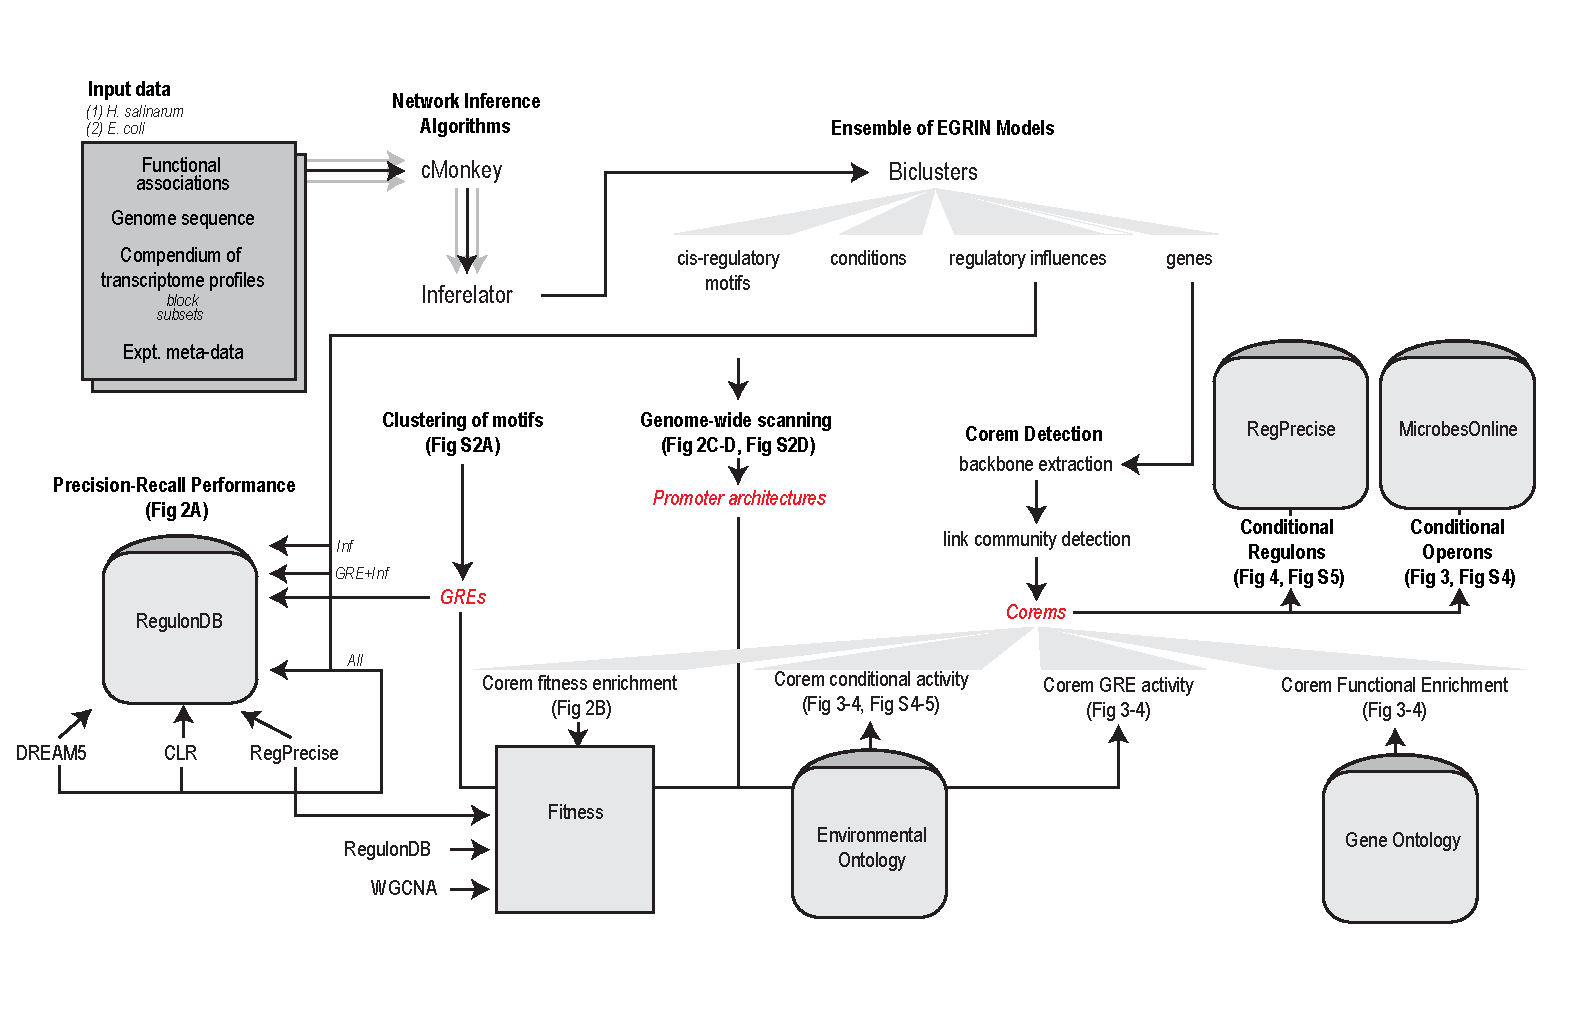
\includegraphics[width=\linewidth]{figures/workflow.pdf}
\caption[Detailed workflow for \egrine~inference procedure]{
{\bf Detailed workflow for \egrine~inference procedure.} Data input,
processing and analysis to construct \egrine~model for {\it
H. salinarum} and {\it E. coli}, and predictions
generated. Predictions highlighted in individual figures are noted.}
\label{fig:workflow}
\end{figure}

%\subsubsection{Statistical mining of the relationships in the ensemble}
\subsubsection{``Ensemble of EGRINs'': generation and statistical mining}

\egrine~model construction and analysis was performed using
primarily the \tmsamp{R} statistical analysis environment, with add-on
packages \tmsamp{data.table} and \tmsamp{filehash} for off-line
storage (maintaining all information in memory was impossible for our
large ensembles). Once the full set of \cm\ and \nwinf\ runs were
completed and stored, a round of post-processing was performed to
agglomerate all results into a single ad-hoc database for storage and
query. The following relationships could be queried to identify
significant associations between biological entities described in the
model:

\begin{tabular}{|l|l|l|r|} 
\hline
Entity$_1$        & Entity$_2$         & Relationship  & Associated info. \\ \hline
Bicluster         & Gene               & Contains      & - \\
Bicluster         & Condition          & Contains      & - \\
Bicluster         & Motif              & Contains      & Associated genes \\
Regulator         & Bicluster          & Regulates     & Weight \\
Motif             & Motif              & Similar       & $FDR\ q$--value \\
Motif             & Genomic coordinate & Overlaps      & $p$-value \\
\hline
\end{tabular}
\\

\noindent These relationships could then be extended to second-degree
relationships, including (these relationships below are by no means
all-inclusive; for brevity we denote $g$, $g_1$, and $g_2$ as separate
genes, $b$ as a bicluster, $m$ as a motif, $r$ as a regulator, and $c$
as an experimental condition):

\begin{enumerate}
\item $g_1$ is co-regulated with $g_2$ if they occur in the same $b$.
\item $g_1$ is co-regulated with $g_2$ under condition $c$ if $g_1$, $g_2$, and $c$ occur in the same $b$.
\item $m$ regulates $g$ if $m$ and $g$ are both observed in the same $b$.
\item $m$ regulates $g$ under condition $c$ if $m$, $g$, and $c$ are all observed in the same $b$.
\item $r$ putatively regulates gene $g$ via $m$ if $r$ is predicted to regulate $b$ which contains both $g$ and $m$.
\end{enumerate}

%% \begin{tabular}{|l|l|l|r|} 
%% \hline
%% Entity$_1$        & Entity$_2$       & Relationship  & Required mapping \\ \hline
%% Gene$_1$          & Gene$_2$         & Co-regulated  & Gene$_1$ and Gene$_2$ in same bicluster \\
%% Gene$_1$          & Gene$_2$         & Co-regulated under condition $C$  & Gene$_1$ and Gene$_2$ in same bicluster \\
%%                   &                  &               & which also contains $C$ \\
%% Gene$_1$          & Motif            & Regulates     & Gene in same bicluster in which Motif was detected \\
%% \hline
%% \end{tabular}

\noindent The frequency with which any of these relationships occurs throughout the
 entire ensemble of EGRIN models could subsequently be counted by
 querying the database, and a $p$-value describing the significance of
 the frequency computed via the cumulative hypergeometric
 distribution. $p$-values were then converted to false discovery rate
 $q$-values using the Benjamini–Hochberg procedure.  We use this
basic procedure to identify conditions associated with GRE influence,
and GREs associated with gene co-regulation, as we describe below.

%% Statistical associations between any entity in the \egrine~ensemble
%% (\ie, genes, GREs, conditions, TFs; see Figure~1) can be evaluated
%% using the hypergeometric test for statistical enrichment.

\subsubsection{Clustering of cis-regulatory motifs to identify GREs}
\label{section:gres}

Each \cm~ bicluster contains at least one {\it de novo} \MEME -
detected \cite{Bailey1998} {\it cis}-regulatory motif. These motifs
are used by \cm~ to guide bicluster optimization (in addition to other
scoring metrics). There were 86,167 and 269,770 motifs detected across
the entire ensemble for {\it E. coli} and {\it H. salinarum},
respectively. Each motif was represented in the model as a
position-specific scoring matrix (PSSM). To determine which of these
motifs represented \textit{bona fide} GREs (as opposed to false positives), we
computed pairwise similarities between all motifs using \tmsamp{Tomtom} 
\cite{Gupta2007} (Euclidean distance metric; minimum overlap of 6 nt) 
and clustered the most highly similar PSSM pairs
using \tmsamp{mcl} \cite{vanDongen2012}. 

The \tmsamp{Tomtom} motif
similarity $p$-value threshold and the \tmsamp{mcl} inflation
parameter ($I$) were selected to (1) maximize the density (unweighted)
of edges between PSSMs inside clusters relative to the edges between
clusters, and (2) ensure that the \tmsamp{mcl} ``jury pruning
synopsis'' was at least 80 (out of 100). Criterion (1) aims to
find a clustering that is as inclusive as possible, while minimizing
over-clustering, while (2) is a built-in mcl metric that evaluates the
quality of the clusters resulting from the user-selected pruning
strategy ($I$). More specifically for criterion (1), we chose the
clustering parameters (\tmsamp{mcl} inflation parameter
$I$, \tmsamp{Tomtom} $p$-value cutoff $p_c$) which maximize:

\begin{equation}
\label{eq:motif:clust}
\left( I, p_c\right) = \arg \max \left\{ \sum_{I=1}^N \sum_{i=1}^{n_I} \frac{ \sum_{j=1}^{n_I} \delta_{ij} }
                            { \sum_{J=1}^N \sum_{k=1}^{n_J} \delta_{ik} } \right\},
\end{equation}

\noindent where $N$ is the total number of motif clusters for a given set of
parameters, $\delta_{ij}$ indicates a significant similarity (subject
to the given $p$-value threshold) the between PSSMs $i$ and $j$ within
motif cluster $I$ (which contains a total of $n_I$ PSSMs), and
$\delta_{ij}$ indicates a significant similarity between PSSM $i$ in
motif cluster $I$ and PSSM $j$ in motif cluster $J$. The final
parameters that maximized expression~\ref{eq:motif:clust} and
resulted in an \tmsamp{mcl} ``jury pruning synopsis'' of at least 80
were different for the two \egrine~models: $p_c = 10^{-6}$
and \tmsamp{mcl} $I = 4.5$ for the {\it H. salinarum} ensemble and
$p_c = 10^{-5}$ and \tmsamp{mcl} $I = 1.5$ for the {\it E. coli}
ensemble.

We did not filter the motifs by $E$-value or other intrinsic motif
quality metrics; rather, we enforced a cluster size threshold to
ensure that GREs were re-detected consistently. Clusters containing at
least 10 PSSMs were considered GREs. This criterion resulted in 135
GREs for {\it H. salinarum} (representing 27,991 PSSMs, Table E2) and
337 for {\it E. coli} (representing 12,773 PSSMs, Table E3). Finally,
we computed a ``combined PSSM'' for each GRE as the unweighted mean of
aligned PSSMs within each cluster. This combined PSSM could be
visualized as a motif logo identically to standard motif PSSMs.

The motif clustering procedure is summarized in Figure \ref{fig:gre_clustering}. 

\begin{figure}[h!]
\centering
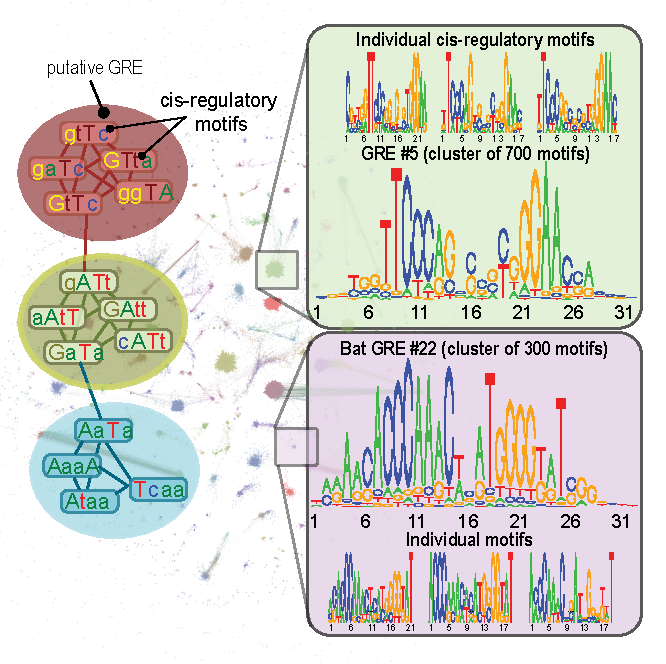
\includegraphics[width=0.6\linewidth]{figures/gre_clustering.pdf}
%\epsfig{file=figures/e2.eps,width=0.8\linewidth}
%\vspace{5in}
\caption[Motif clustering and GRE identification]{
\textbf{Motif clustering and GRE identification.} 
(Left) A schematic of the approach used to align and cluster
individually detected motifs to define GREs. In this example, similar
motifs were aligned and clustered into three GREs using Tomtom and mcl
(Details in Methods and Supplementary Methods). (Center) The {\it
H. salinarum} network of aligned and clustered motifs. (Right) Two
{\it H. salinarum} GREs discovered by this method. The motif logo of
each GRE was generated by summing PSSMs of the individual aligned
motifs in the cluster, as illustrated by three examples of individual
motifs (prior to alignment) for each of the two GREs. Note that
relative to the individual motifs, the averaged GRE motif is more
palindromic - a hallmark of binding sites for dimeric TFs.}
\label{fig:gre_clustering}
%\vspace{-.1in}
\end{figure}

\subsubsection{Genome-wide scanning of motifs to obtain GRE locations}
\label{section:scanning}

We used motif scanning to discover GRE locations that were missed by
the rigid definition of a promoter in \cm\ (typically -250 to +50
nucleotides surrounding the translation start site). This procedure
was critical for discovering GREs in non-canonical locations, such as
internal to operons. We computed how well each PSSM (described above)
matched every position in the genome
using \tmsamp{MAST} \cite{Bailey1998}, and recorded significant
matches at each genomic location subject to a position $p$-value
threshold of $10^{-5}$. This $p$-value cutoff corresponds to an
expectation of discovering $\sim 20$ sites at random across the
genome. For each GRE, we summed the number of significant matches to
each of the GRE’s PSSMs at each genomic position. These counts were
used to represent GRE composition in promoters (Figures~2-3). In
addition, we used these scanned locations to identify GREs located
predominantly inside coding regions. Since these GREs may be spurious
(\eg, protein sequence motifs or trinucleotide patterns) they were
flagged, although they were not removed from our global analysis.

We compared the genome-wide distribution of GRE locations to annotated
start sites in \textit{H. salinarum}.  We discovered that most GREs
occur in consistent locations with respect to gene start sites.  The
global position of all GREs and select GREs relative to experimentally
determined gene start sites is depicted in
Figure \ref{fig:gre_global_locs_hal}.

\begin{figure}[h!]
\centering
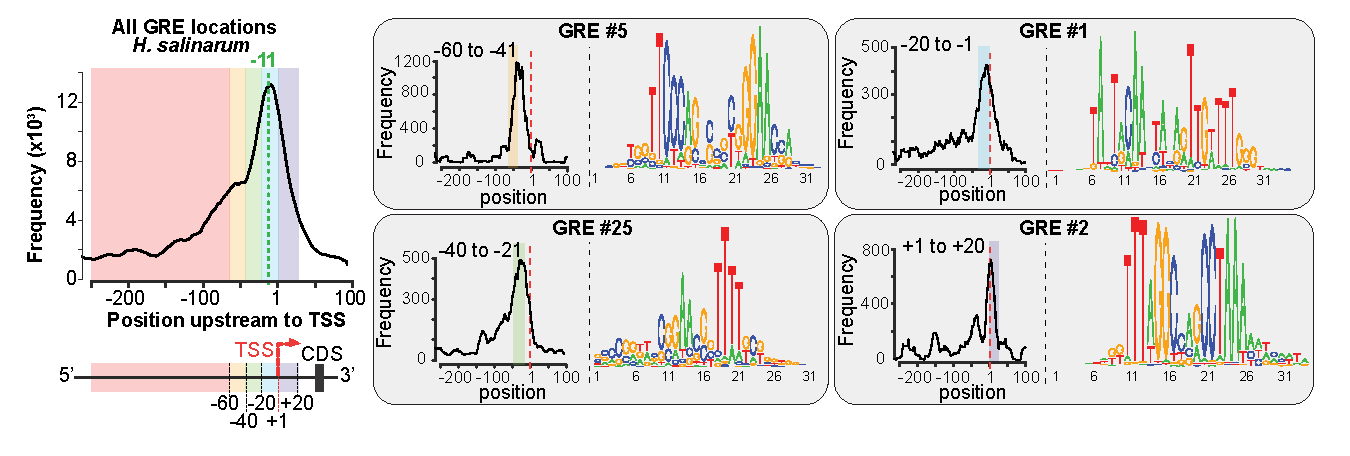
\includegraphics[width=0.95\linewidth]{figures/gre_global_locs_hal.pdf}
\caption[Genome-wide distribution of GREs relative to experimentally mapped 
transcriptional start sites in \textit{H. salinarum}]{
\textbf{Genome-wide distribution of GREs relative to experimentally 
mapped transcriptional start sites in \textit{H. salinarum}.}  (Left)
Predicted positions for all GREs in gene promoters upstream of
experimentally mapped transcription start sites
(TSSs; \cite{Koide2009}) in and (Right) four example
elements. Distribution peaks for most GREs occur at characteristic
locations. For instance, the location of TATA box-like elements
(GRE \#25) between -21 to -40 nt upstream to TSSs in {\it
H. salinarum} is consistent with the characterized location of basal
elements in archaeal promoters (-25 to 30 nt upstream to TSS). GRE
location enables prediction of putative roles for the cognate TF (\eg
repressor, activator or a basal factor).}
\label{fig:gre_global_locs_hal}
\end{figure}



\subsubsection{Identifying corems}

\paragraph{Gene-gene co-occurrence network}
\label{section:gBg}

We post-processed the \egrine~ensemble to refine the underlying
network structure and discover functionally meaningful gene
co-regulatory modules present in the model. To do so, we transformed
the ensemble of biclusters into a weighted gene-gene association graph
$G$, where the nodes of $G$ are genes and the weight of edges between the
nodes is proportional to their frequency of co-occurrence in
biclusters:

\begin{equation}
w_{ij} = \frac{\left|B_i\cap B_j\right|}{\mathrm{min}(B_i,B_j)},
\end{equation}

\noindent where $w_{ij}$ is the weight of the edge between genes $i$ and $j$,
$B_i$ is the set of all biclusters containing gene $i$. The weights
were normalized by the minimum number of biclusters containing either
gene, rather than by the more typically applied union (which would
make the score identical to the Jaccard Index) to avoid penalizing
genes that occur infrequently in biclusters. The sum of edge weights
for each gene was normalized to one. This gene-gene co-occurrence
network represents how often \cm~ discovers co-regulation between
every pair of genes in the genome. We note that since this network is
derived from biclusters, it is also a reflection of conditional
co-expression and predicted \textit{cis}-­regulatory motifs.

\paragraph{Network backbone extraction}

After transforming the ensemble into a normalized graph, we removed
edges that were statistically indistinguishable by multiscale backbone
extraction (null hypothesis of uniform edge weight distribution given
a node of degree $k$) \cite{Serrano2009}. We retained all edges
satisfying the following relation:

\begin{equation}
\alpha_{ij}=1-(k-1)\int_0^{w_{ij}}(1-x)^{k-2}dx\leq 0.05,
\end{equation}

\noindent where $\alpha_{ij}$ is the probability that the normalized weight $w_{ij}$ between
genes $i$ and $j$ is compatible with the null hypothesis, and $k$ is
the degree of gene $i$. For \halo, backbone extraction reduced the
number of regulatory edges from 1,576,643 to 141,667; in \eco~ the
number of edges was reduced from 3,094,954 to 170,723.

\paragraph{Network link-community detection}
\label{section:linkcommunity}
Following backbone extraction, we detected corems by application of a
recently described link-community detection
algorithm \cite{Ahn2010}. For this algorithm to work on our data set
we modified it to accept input of a weighted graph \cite{Kalinka2011}.
We implemented it in \tmsamp{C++} for efficiency. The algorithm
computes a similarity score between all pairs of edges sharing a
common keystone node, $k$, according to the Tanimoto coefficient, $T$:

\begin{equation}
T(e_{ik},e_{kj}) = \frac{a_i\cdot a_j}{|a_i|^2+|a_i|^2+a_i\cdot a_j},
\end{equation}

\noindent where

\begin{equation}
a_i=w_{ij}+\frac{\delta_{ij}}{k_i}\sum_{l\in n(i)}w_{il}.
\end{equation}

\noindent Here, $e_{ik}$ is the edge between gene $i$
and the keystone gene $k$, and $\delta_{ij}$ is the Kroenecker delta. The score
reflects the similarity of gene neighborhoods adjacent to two edges
sharing a gene, with the score increasing in value as the number and
weight of overlapping adjacent edges increases. To transform the
Tanimoto coefficient into a distance metric, we compute $1-T$.

Following scoring, the edges were aggregated by standard hierarchical
clustering. The resulting tree is cut at many thresholds to optimize
the local weighted density $D$ of the resulting clusters:

\begin{equation}
D=\frac{1}{M\langle w\rangle}\sum_{c\in C}m_c\langle w\rangle_c\left(\frac{m_c-(n_c-1)}{n_c(n_c-1)/2-(n_c-1)}\right),
\end{equation}

\noindent where $M$ is the total number of edges in the
entire network, $\langle w\rangle$ is the average weight of edges in the entire
network, $C$ is the set of all link communities at a given threshold, $m_c$
is the number of edges in community $c$, $\langle w\rangle_c$ is the average weight of
edges in community $c$, and $n_c$ is the number of genes in community
$c$. The density scoring metric $D$ had a clear optimum corresponding exactly to
the cutoff that would have been chosen had we used the unweighted
scoring metric originally described (Figure \ref{fig:corem_density}). Only
communities with more than two genes were retained.

\begin{figure}[hp]
\centering
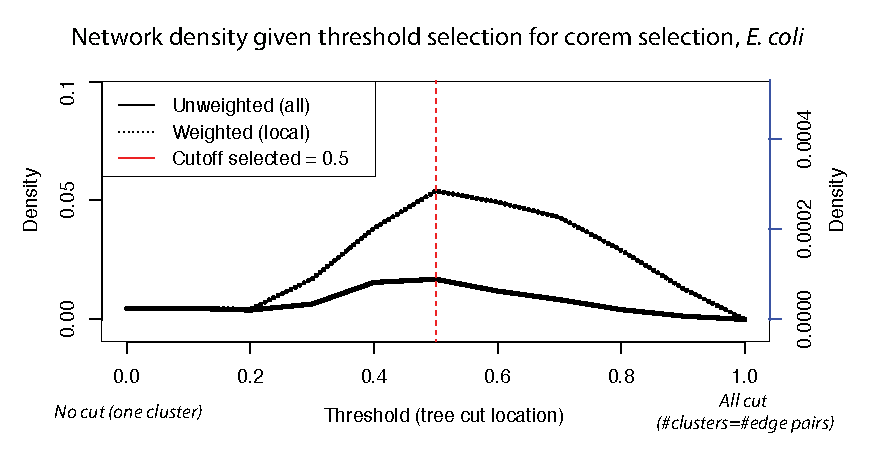
\includegraphics[width=0.9\linewidth]{figures/corem_density.pdf}
\caption[Corem density as a function of clustering cutoff threshold]{
{\bf Corem density as a function of clustering cutoff threshold.}
Hierarchical clustering cut threshold chosen to maximize the density
of resulting clusters. The cutoff chosen with modified weighted
density metric is identical to unweighted density metric.}
\label{fig:corem_density}
\end{figure}

Since the communities produced by this algorithm are comprised of sets
of edges, we defined a corem to include all genes incident to the
edges in a community. Because of this definition, each gene can be a
member of multiple different corems. In {\it H. salinarum}, this
procedure generated 679 corems ranging in size from 3 to 377 genes,
covering 1,363 of the 2,400 genes in the genome, and comprising 56,738
co-regulatory associations. In {\it E. coli}, we discovered 590
corems, ranging in size from 3 to 153 genes, covering 1,572 of 4,213
genes and 25,976 regulatory edges. See Table E1 and
Figure \ref{fig:corem_density} for additional
statistics. Gene-to-corem and corem-to-gene mappings for the {\it
H. salinarum} and {\it E. coli} models are available online.

\begin{figure}[hp]
\centering
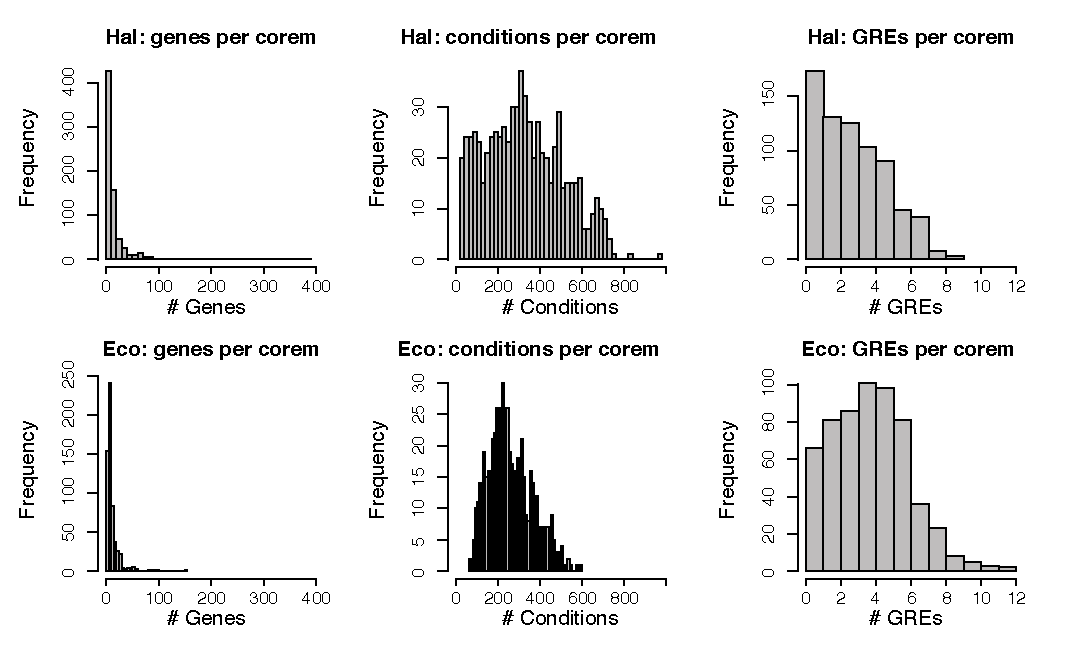
\includegraphics[width=0.9\linewidth]{figures/corem_stats.pdf}
\caption[Corem statistics]{
{\bf Corem statistics.} Number of genes, conditions, and GREs per
corem for \textit{E. coli} and \textit{H. salinarum} \egrine~models.}
\label{fig:corem_stats}
\end{figure}


\subsection{Functional enrichment estimates for genes in corems}

We computed functional enrichment for genes organized into corems
using \DIFdelbegin \DIFdel{DAVID (Dennis et al., 2003) and the
DAVIDQuery R-package (Day
and Lisovich, 2010)}\DIFdelend \DIFaddbegin \tmsamp{DAVID} \DIFadd{\mbox{%DIFAUXCMD
\cite{Dennis2003}
}%DIFAUXCMD
and the
}\tmsamp{DAVIDQuery} \DIFadd{\mbox{%DIFAUXCMD
\cite{Day2010}
}%DIFAUXCMD
}\tmsamp{R}\DIFadd{-package}\DIFaddend . Enrichments for each corem are available on the
\DIFdelbegin \DIFdel{web site}\DIFdelend \DIFaddbegin \href{http://egrin2.systemsbiology.net}{web site}\DIFaddend .

\subsection{Conditional co-regulation of genes organized in corems}
\DIFaddbegin \label{section:rsd}
\DIFaddend 

We defined the conditions in which genes in a corem were co-regulated
as the set of experiments in which the genes of a corem are more
tightly co-expressed than one would expect at chance. We statistically
evaluated tight co-expression using relative standard deviation (RSD 
$=|\sigma/\mu|$) \DIFdelbegin \DIFdel{and }\DIFdelend \DIFaddbegin \DIFadd{by }\DIFaddend resampling. We chose RSD (rather than, for example,
standard deviation, $\sigma$) to avoid over-weighting conditions in which the
mean relative expression is close to zero. The significance of an RSD
value for a given condition relative to each corem was estimated
by resampling: for a corem with $k$ gene members, and for each
condition, $c$, we computed at least 20,000 RSD values for $k$ randomly
sampled expression measurements in $c$, to determine the likelihood that the
observed co-expression has lower RSD than expected by chance ($p$-value
$< 0.01$). The resampling procedure resulted in condition sets for
corems that contained from 1.4\% to 85.5\% of the conditions in
\halo\ and 7.9\% to 66.6\% conditions in \eco\DIFaddbegin \ \DIFadd{(Figure \ref{fig:corem_stats})}\DIFaddend .

\subsection{Conditionality of GRE influence}

The upstream promoter regions of most genes contain multiple EGRIN
2.0-predicted GREs (\eg, \DIFdelbegin \DIFdel{carA }\DIFdelend \DIFaddbegin \textit{\DIFadd{carA}} \DIFaddend in Figure 2). A key insight of our model
is that not all of these sites are equally important for controlling
gene expression in all experimental conditions. We refer to changes in
the relative influence of GREs across conditions as \DIFdelbegin \DIFdel{“conditional
activity�}\DIFdelend \DIFaddbegin \DIFadd{``conditional
activity'' }\DIFaddend of GRE elements. Although, to be clear, we do not imply
that the transcriptional activity at a GRE is attributable to the DNA
sequence itself, but rather the TF that binds to that sequence in
particular environments. We leveraged the GREs discovered in genes
grouped into corems and the conditional co-expression of those groups
of genes to predict conditionally active GREs in \DIFdelbegin \DIFdel{EGRIN
2.0}\DIFdelend \DIFaddbegin \egrine\DIFaddend .

\DIFdelbegin \DIFdel{Specifically, to discover }\DIFdelend \DIFaddbegin \DIFadd{To identify the }\DIFaddend active GREs for each corem we combined predictions
from (1) genome-wide motif scans (Section\DIFdelbegin \DIFdel{5 }\DIFdelend \DIFaddbegin \DIFadd{~\ref{section:scanning}
}\DIFaddend above) that predict the GRE locations in an expanded region around
each gene’s promoter in the corem using all of the ensemble
predictions (1,000 nt window: -875 nt upstream to 125 nt downstream),
and (2) the conditions discovered in biclusters that are most
representative of the corem (\ie, containing the largest fraction of
genes from the corem, top decile). GREs that occurred frequently
\DIFdelbegin \DIFdel{in }\DIFdelend \DIFaddbegin \DIFadd{in }\DIFaddend these biclusters were considered putatively responsible for
co-regulating the set of genes in the condition-specific context of
the corem (\DIFdelbegin \DIFdel{q-value ≤
}\DIFdelend \DIFaddbegin \DIFadd{$q$-value $\leq$ }\DIFaddend 0.05). Finally, we computed the average distances
of all GREs to the start codons of each gene in the list (collapsing
sites if they occurred within 25 nt of one another). The precise
locations of all GREs for the {\it H. salinarum} \DIFdelbegin \DIFdel{dpp }\DIFdelend \DIFaddbegin \textit{\DIFadd{dpp}} \DIFaddend operon-related
corems (Figure 3) are listed in Table E8, while the locations \DIFdelbegin \DIFdel{for }\DIFdelend \DIFaddbegin \DIFadd{of }\DIFaddend GREs
involved in conditional modulation of the PurR regulon (Figure 4) are
provided in Table E9.

We represented the active GREs upstream of a gene or within a corem as
a pie chart, showing the normalized frequency with which the GREs
computed above occurred in biclusters containing that gene. For
example, if GREs 1, 2, and 3 occurred in 25, 50, and 200 biclusters
containing gene \DIFdelbegin \DIFdel{A}\DIFdelend \DIFaddbegin \DIFadd{$A$}\DIFaddend , the pie chart for gene \DIFdelbegin \DIFdel{A }\DIFdelend \DIFaddbegin \DIFadd{$A$ }\DIFaddend would have sectors of area
0.09, 0.18, and 0.73 respectively. For corems, we computed the
normalized frequency of GREs for all genes of the corem. For example,
if GREs 1, 2, and 3 occurred in promoters of 10, 10, and 20 of the
genes of the corem, their areas would be 0.25, 0.25, and 0.5
respectively.

\DIFdelbegin \subsection{\DIFdel{Detection of conditional operons}}
%DIFAUXCMD
\addtocounter{subsection}{-1}%DIFAUXCMD
\DIFdelend \DIFaddbegin \begin{figure}[hp]
\centering
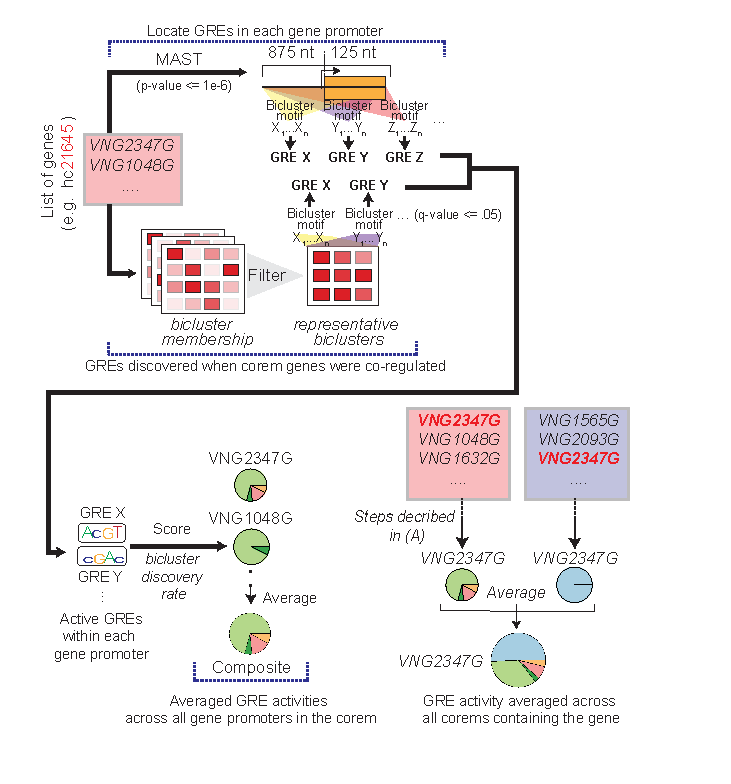
\includegraphics[width=0.95\linewidth]{figures/corem_gres.pdf}
\caption[Deciphering GREs responsible for regulating corems]{\textbf{\DIFaddFL{Deciphering GREs responsible for regulating corems.}} \DIFaddFL{A GRE is implicated in regulation of a corem when it is both (1) located within an expanded region (-875nt to +125nt) around the translation start site of any gene in the corem; and (2) present in biclusters containing a large fraction of corem genes (top decile). Relative GRE influence is computed as the frequency with which each GRE was discovered in these representative biclusters (see Supplementary Methods for more details). Influence scores are illustrated as pie charts and reported for each gene individually (}\eg\DIFaddFL{, }\textit{\DIFaddFL{VNG2347G}}\DIFaddFL{); and as a composite by averaging across all genes in a corem. The width of each sector in the pie charts is proportional to the frequency of GRE discovery.}}
\label{fig:corem_gres}
\end{figure}
\DIFaddend 

\DIFdelbegin \DIFdel{Conditional-specific }\DIFdelend \DIFaddbegin \subsection{\DIFadd{Detection of conditional operons}}
\label{section:condop}
\DIFadd{Condition-specific }\DIFaddend transcriptional isoforms of operons were predicted
through corem membership. \DIFdelbegin \DIFdel{Specifically, if }\DIFdelend \DIFaddbegin \DIFadd{If }\DIFaddend any of the genes in an operon were found
in a corem that did not contain all the other genes of the operon, we
predicted that the operon had conditional isoforms. Operon annotations
for both {\it H. salinarum} and {\it E. coli} were derived from
\DIFdelbegin \DIFdel{MicrobesOnline}\DIFdelend \DIFaddbegin \tmsamp{MicrobesOnline} \DIFadd{\mbox{%DIFAUXCMD
\cite{Alm2005,Price2005b}
}%DIFAUXCMD
}\DIFaddend . All predicted conditional
operons, including the specific break sites and transcriptional
isoforms is available on the website. The full list of validated
predictions is provided in Table E7.

\subsection{Environmental ontology construction and usage}

We recorded a rich \DIFdelbegin \DIFdel{meta-data set for all 1495 experiments
conducted for }\DIFdelend \DIFaddbegin \DIFadd{set of meta-data for all 1,495 experiments
conducted with }\DIFaddend {\it H. salinarum} \DIFaddbegin \DIFadd{and used for construction of the
}\halo\DIFadd{~ }\egrine\DIFadd{~model}\DIFaddend . The meta-data includes a detailed description
of each experiment, including, for example: media composition, genetic
background, concentration of perturbant, internal reference batch id,
person who conducted the experiment, etc. We used this
meta-information to classify experiments in an ontological framework,
where two experiments can share specific meta-descriptions (\eg,
\DIFdelbegin \DIFdel{1e-3
}\DIFdelend \DIFaddbegin \DIFadd{$10^{-3}$ }\DIFaddend mol/L EDTA), or inherit more general relationships from the
ontological structure (\eg, chemical perturbation). We used OBO-edit
\DIFaddbegin \DIFadd{\mbox{%DIFAUXCMD
\cite{Day-Richter2007}
}%DIFAUXCMD
}\DIFaddend to construct the ontology. The ontology contained 198
terms organized across three primary branches (environmental state,
experimental state, and genetic state). The ontology flat file is
available for download and meta-data annotations for every array in
the dataset are available \DIFdelbegin \DIFdel{online}\DIFdelend \DIFaddbegin \href{http://egrin2.systemsbiology.net}{online}\DIFaddend .

We used the ontology to classify enriched environmental features for
GREs and corems (Figures 3-4). For corems, we used the set of
conditions in which genes in the corem are significantly co-expressed
(see \DIFdelbegin \DIFdel{9 }\DIFdelend \DIFaddbegin \DIFadd{Section \ref{section:rsd} }\DIFaddend above) to compute term enrichment using the \DIFdelbegin \DIFdel{ontoCAT
R-package}\DIFdelend \DIFaddbegin \tmsamp{ontoCAT}
\DIFadd{\mbox{%DIFAUXCMD
\cite{Kurbatova2011}
}%DIFAUXCMD
}\tmsamp{R}\DIFadd{-package}\DIFaddend . Term enrichment was assessed
statistically and reported as \DIFdelbegin \DIFdel{q-values }\DIFdelend \DIFaddbegin \DIFadd{$q$-values }\DIFaddend using the hypergeometric test
with Benjamini-Hochberg correction for multiple hypothesis testing.
\DIFaddbegin 

\begin{figure}[hp]
\centering
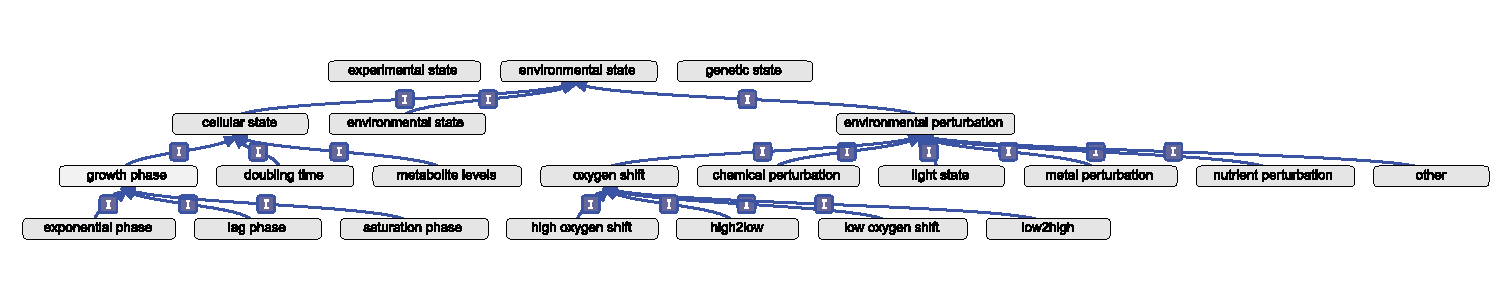
\includegraphics[width=0.9\linewidth]{figures/eo.pdf}
\caption[Environmental ontology hierarchically organizes relationships between experimental conditions from metadata collected across 1495 experiments in \textit{H. salinarum}]{{\bf \DIFaddFL{Environmental ontology hierarchically organizes relationships between experimental conditions from metadata collected across 1495 experiments in }\textit{\DIFaddFL{H. salinarum}}\DIFaddFL{.}} \DIFaddFL{Subset of the environmental ontology constructed for }\textit{\DIFaddFL{H. salinarum}} \DIFaddFL{demonstrates many “is-a” (boxed ‘I’) relationships that organize similarities between descriptor terms descending from one of three root nodes (i.e., generic categorical descriptions). In this case a generic ontological term called `environmental state' gives rise to much more specific terms (e.g., exponential phase or high oxygen shift) that inherit (at the highest level) a relationship through their being related to the ‘environmental state’ of cells in the experiment. Each condition in the compendium is annotated with the most specific descriptors relevant to the experiment given metadata. Mapping of arrays to ontology terms is provided in Supplementary Table 3. The full environmental ontology is available for download from }\href{http://egrin2.systemsbiology.net}{http://egrin2.systemsbiology.net}\DIFaddFL{.}}
\label{fig:eo}
\end{figure}
 \DIFaddend

\section{Model validation}\label{sec:validation}

\subsection{Global validation of gene regulatory elements predicted by \egrine}
\label{section:tfbs:vs:regdb}

We compared the genome-wide locations of predicted GREs in the {\it
  E. coli} \egrine~model to experimentally mapped TF binding sites
from \rdb~(BindingSiteSet table, filtered for experimental evidence
and TFs with $\geq 3$ unique binding sites; a total of 88 TFs). We
considered a GRE to be a significant match to a TF if a significant
fraction ($q$-value $\leq 0.05$) of its predicted non-coding locations
overlapped with the known binding locations for a particular TF
(hypergeometric $p$-value $\leq 0.01$; see GRE definition in
Section~\ref{section:gres}). In cases where a GRE significantly
matched multiple TFs, only the most significant was reported.

We observed several instances where more than one GRE significantly
matched the same TF. We were unable to determine whether this was the
result of incomplete GRE clustering, ambiguities related to GRE
scanning, limitations of the experimental data itself, or a reflection
of subtle context-dependent variations in the binding preferences of
these TFs. Since we did not observe clustering of GREs that map to the
same TF upon re-clustering, we hypothesize that the observations may
have biological origins, \ie, reflect condition-dependent variations
in TF binding preferences that are the result, for example, of
co-activator/repressor interaction or small molecule binding. It is
interesting to note that TFs with the largest fraction of GRE matches
include transcriptional dual regulators, such as FlhDC and UlaR (\ie,
TFs with the ability to act as both activators and repressors). This
is consistent with the observation that these TFs have
context-dependent binding preferences. The complete set of
validations, for both TFs and $\sigma$-factors, is listed in Table~E4.

\subsection{Global validation of regulatory interactions predicted by \egrine}
\label{section:aupr:vs:regdb}

We assessed the ability of the \egrine\ model to correctly infer known
regulatory interactions using the \rdb\ database as a standard metric
for comparison. Comparison to the \rdb\ gold-standard is common
practice for evaluating model performance \cite{Marbach2012}. We
performed our evaluation with the version of \rdb~ used by the DREAM5
ensemble (based on \rdb\ release 6.8 \cite{Marbach2012}) so that we
could directly compare our results. The authors \cite{Marbach2012}
restricted the gold-standard to well-established interactions,
annotated in \rdb\ with the `strong evidence' classification. In all
cases, networks were integrated from predictions among the ensemble
using an approach similar to that of \cite{Marbach2012}, with subtle
variations noted in each section, below. To facilitate a direct
comparison, we reconstructed a new {\it E. coli} \egrine\ model using
the same DREAM5 expression consortium as was used for the original
DREAM5 competition (Section~\ref{section:dream5_data_compendium}). The
predictions of this model were used {\it solely} for global validation
and direct comparison with the DREAM5 community network, as described
in this subsection.

We performed two global evaluations of the {\it E. coli} \egrine: (1)
a comparison of the GREs detected in the model with experimentally
mapped TF binding sites in \rdb~(Section~\ref{section:tfbs:vs:regdb}),
and (2) a comparison of the predicted (TF $\rightarrow$ gene) regulation
in \egrine~with the gene regulatory network from
\cite{Marbach2012}. For (2), we computed predicted regulatory networks
from \egrine~in two ways: (a) direct (TF $\rightarrow$ target)
predictions from \nwinf~ (Section~\ref{sec:nwinf_network}, and (b) a
gene regulatory network derived from predicted GREs that were matched
to TFs in
\rdb~(Section~\ref{section:gre_grn_construction}). Construction of
each of these networks is described in detail below
(Section~\ref{sec:nwinf_network} and
Section~\ref{section:gre_grn_construction}). The methods for, and
results of the comparisons are described in
Section~\ref{sec:network_comparisons}.

\subsubsection{Conversion of \egrine~\nwinf~influence predictions into a GRN}
\label{sec:nwinf_network}

We computed a direct (TF $\rightarrow$ gene) inferred {\it E. coli}
gene regulatory network (GRN) from the \nwinf~predictions in the
\egrine~ensemble. As with the original EGRIN model \cite{Bonneau2007},
\nwinf~influence predictions were originally made between the 296
putative {\it E. coli} TFs (Section \ref{section:eco_tfs}) and each of the
$\sim 40,000$ biclusters in the ensemble. We then used a weighted
average of the predicted influences among all networks in the
ensemble, as follows. If \nwinf~predicted a (TF $\rightarrow$
bicluster) influence with weight $\beta$ then we added $\beta$ to a
regulatory interaction between that TF and all genes in that
bicluster. Weights $\beta$ were summed for each recurrence of the same
(TF $\rightarrow$ gene) interaction. Note, we did not use $|\beta|$ in
the individual sums, since we considered contradicting evidence to be
cancelling rather than reinforcing. Finally, all (TF $\rightarrow$
gene) interactions in the final network were ranked by absolute total
weight (here we {\it did} use $|\beta|$). As with the DREAM5
competition networks, the top 100,000 rankings were retained in the
final network. The final \egrine~\nwinf~influence network is available
\href{http://egrin2.systemsbiology.net/}{online}.
%at \ref{tables:Inferelator_network.tsv}.

\subsubsection{Conversion of \egrine~GRE detections into a predicted GRN}
\label{section:gre_grn_construction}

We computed a separate inferred {\it E. coli} gene regulatory network
from predicted GREs in \egrine\ that were matched to TFs as described
in Section~\ref{section:tfbs:vs:regdb}. We would like to stress that
this inference relies upon (in this case, for {\it E. coli}) annotated
binding sites for regulators, which could be statistically linked to
predicted GREs through significant overlaps in their genomic
locations. This enables inference of (TF $\rightarrow$ gene) direct
influence predictions through the indirect relationship: 

\begin{equation}
\label{eq:gre_network_relation}
\mathrm{TF} \overset{\mathrm{anno.}}{\rightarrow} \mathrm{GRE} \overset{\mathrm{pred.}}{\rightarrow} \mathrm{gene}.
\end{equation}

\noindent Thus for an understudied organism, such as {\it
  H. salinarum}, such a network of (TF $\rightarrow$ gene) influences
could {\it not} be inferred; rather a (GRE $\rightarrow$ gene)
interaction network would be the final product. Such a network still
contains predictions which could be validated and acted upon, for
example, for engineering purposes. A future direction of our research
will be to statistically link TFs to predicted GREs, for example using
direct GRN predictions such as those described above
(\eg\ Section~\ref{sec:nwinf_network}, or \cite{Marbach2012}).

(GRE $\rightarrow$ gene) predictions (in
Eq.~\ref{eq:gre_network_relation}) were extracted from the
\egrine\ model directly using the \MEME\ predictions for motif
instances in the promoters of genes in each of the $\sim$40,000
\cm\ biclusters. We then used an unweighted average of the predictions
among all bicluster in the ensemble, as follows. A (TF $\rightarrow$
gene) edge with a weight of 1 was added to the predicted network if
the annotated binding sites for that TF could be matched with
locations of a motif (Section \ref{section:tfbs:vs:regdb}), which was
detected by \MEME\ in a bicluster in the promoter of the gene. Edge
weights (1) were added for each additional prediction, in the ensemble
of biclusters, of the same (TF $\rightarrow$ gene) interaction. As
with the \nwinf~influence network (Section \ref{sec:nwinf_network}), the top
100,000 rankings were retained in the final network. The final
\egrine~GRE-based network is available 
\href{http://egrin2.systemsbiology.net/}{online}.
%at \ref{tables:GRE_network.tsv}.

\subsubsection{Integration of predicted \egrine~\nwinf- and GRE-based GRNs}

Prior to integration of the two different predicted GRNs described
above (Sections~\ref{sec:nwinf_network}
and~\ref{section:gre_grn_construction}), we ensured that they were
both equally represented in the integrated GRN by re-scaling their
weights so that their sums would be equal. The GRNs were then combined
into a single, integrated predicted \egrine\ GRN by simply summing the
re-scaled weights for any edge predicted in both networks. Thus, this
final network integration was a form of weighted average of the two
(GRE and \nwinf) networks. This is {\it not} identical to the weighted
rank average method described by \cite{Marbach2012}, as it does not
use a posteriori assessments of each network to assign their relative
weights; rather the weights are simply adjust so that each network
contributes equally to the predictions.

\subsubsection{Network comparisons and global performance assessments}
\label{sec:network_comparisons}

To compare \egrine\ performance to the DREAM5 ensemble, we computed
standard precision-recall statistics for each network using the
previously described DREAM5 gold standard GRN.  We computed
area-under-the-precision-recall (AUPR) statistics to summarize the
predictive performance. AUPR statistics were compared directly with
the DREAM5 community ensemble network. By extension, the \egrine~AUPR
performance can be compared to the individual best performers in
DREAM5 as well (Figure~2A in \cite{Marbach2012}). The results of these
analyses are summarized in Figure~2A in the main text. We have made
all network predictions available
\href{http://egrin2.systemsbiology.net/}{online}. Complete
precision-recall curves are shown in Figure~\ref{fig:pr_curves}. The
curves are also available in tabular form
\href{http://egrin2.systemsbiology.net/}{online}.

\begin{figure}[h!]
\centering
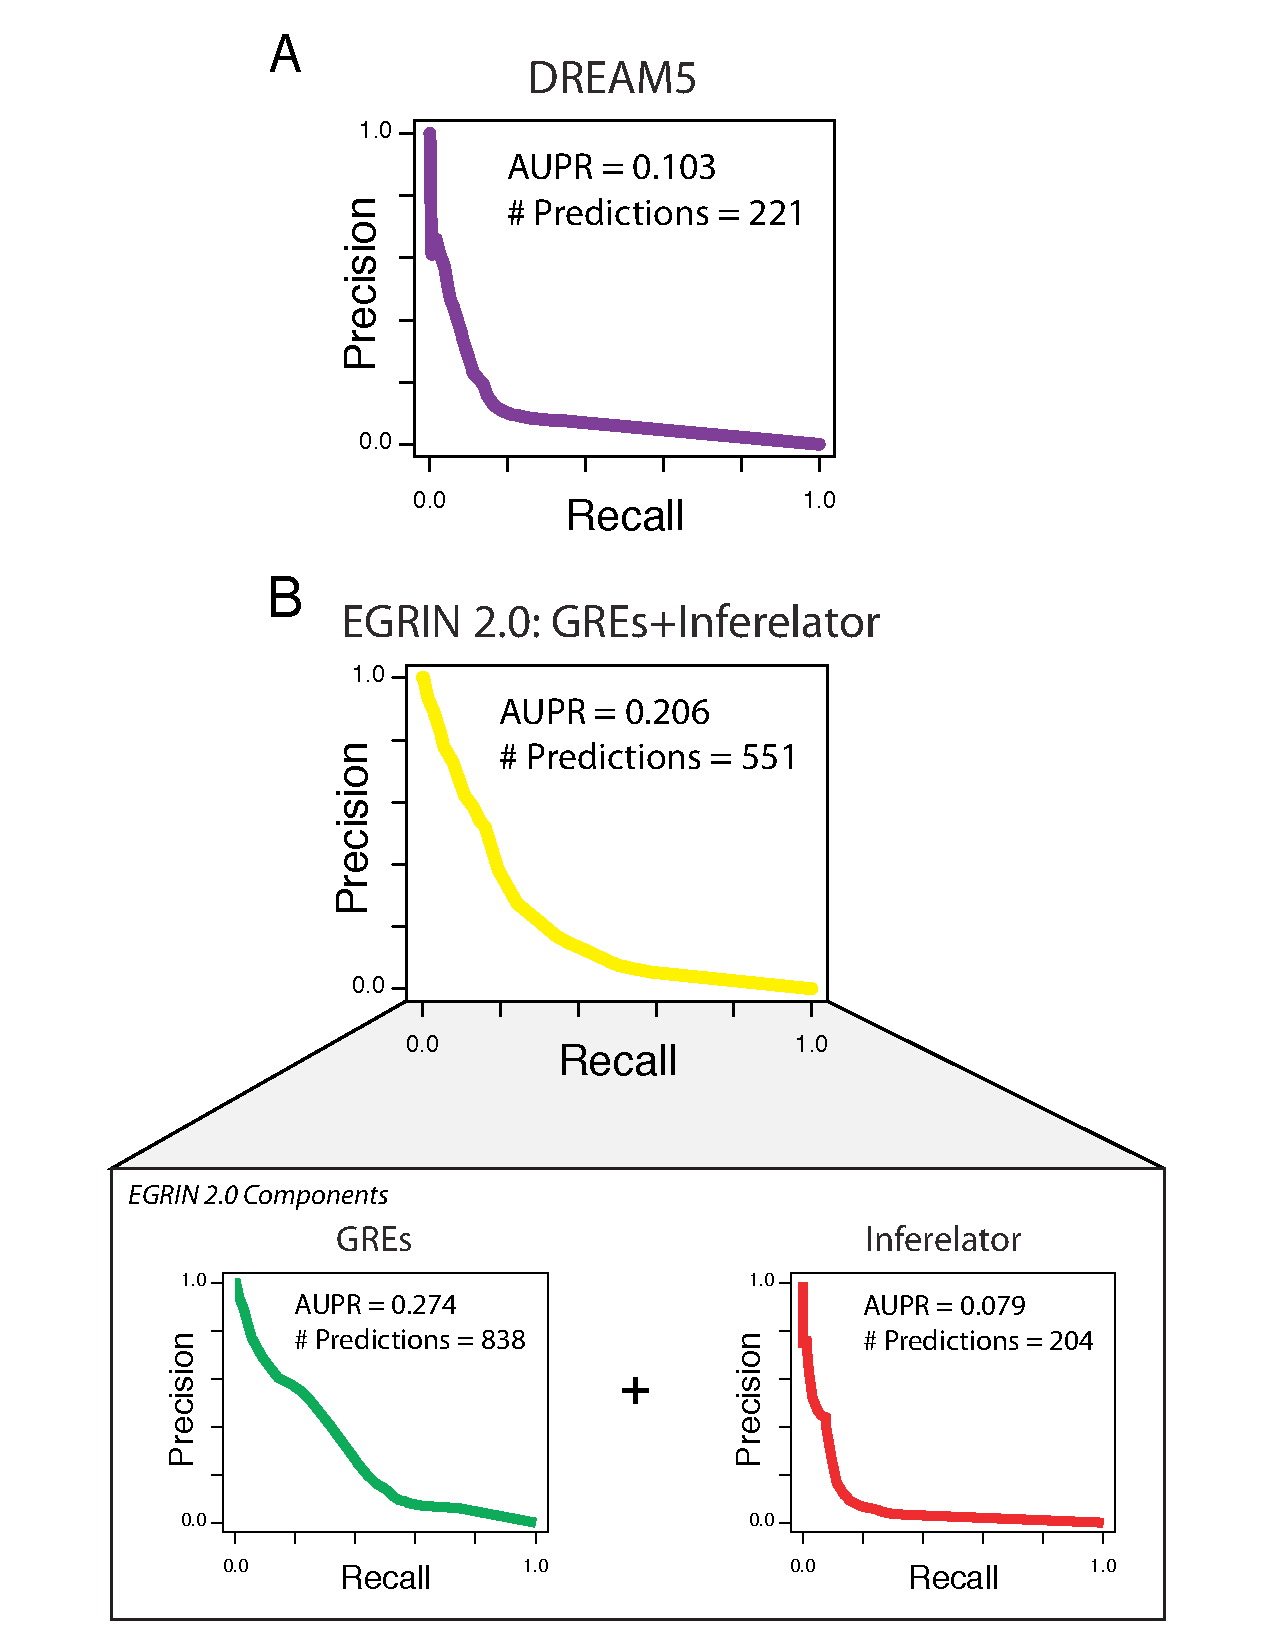
\includegraphics[width=0.5\linewidth]{figures/aupr.pdf}
\caption[Precision-recall performance for {\it E. coli}
  networks.]{\textbf{Precision-recall performance for \textit{E. coli}
    networks.} Comparison of precision-recall performance on {\it
    E. coli} \rdb~gold-standard (Section
  \ref{section:eco:gold:standard}), for the DREAM5 ensemble network
  (A), compared to \egrine (B).  We compare the GRE-based and
  \nwinf-based networks (bottom)to the integrated \egrine~network
  (top). The integrated \egrine~network consists of an equal weighting
  of the GRE-based and \nwinf-based networks.  The \egrine~networks
  were inferred using the DREAM5 mRNA expression compendium (Section
  \ref{section:dream5_data_compendium}). Area under the curve (AUPR)
  and the number of true-positive predictions at a precision of 25\%
  are listed for each curve.}
\label{fig:pr_curves}
\end{figure}

We further investigated the convergence of the AUPR statistics for
each of the \egrine-predicted regulatory networks as additional
individual EGRIN models are added to the ensemble. This assessment
helps to address the question of whether the approach utilized for
ensemble integration has the desired property of performing better
than most (if not all) of the individual models. Additionally, it can
address the question of how many individual EGRIN models are necessary
to achieve a given performance level. We observed that this is indeed
the case for the \nwinf-based predictions extracted from the
\egrine\ model (Figure~\ref{fig:cumulative_auprs}a), whose final AUPR
of 8.5\% far exceeds the rather poor performance of all 106 individual
component EGRIN models (with an average AUPR of 5.0\% and a maximum of
7.4\%). The performance of the ensemble for this measure converges
rather quickly to the final measure, after roughly 50 of the 106 EGRIN
models are integrated (taking into account the variance in models
observed with integrating the models in different orders).  For the
\egrine\ GRE-based predicted network
(Figure~\ref{fig:cumulative_auprs}b), ensemble surpasses 84 (79\%) of
the 106 individual component EGRIN models. This measure continues to
improve until $\sim 80$ of the 106 models are integrated, suggesting
that for this data set (the DREAM5 {\it E. coli} expression
compendium), $\sim 100$ EGRIN models was a reasonable number to use in
construction of the \egrine\ ensemble.

\begin{figure}[hp]
\centering
\mbox{
\subfigure[]{\includegraphics[width=0.4\linewidth]{figures/nwInf_cumulative_forPaper.pdf}}
\subfigure[]{\includegraphics[width=0.4\linewidth]{figures/motif_cumulative_forPaper.pdf}}
}
\caption[Ensemble performance of individual GRN predictions]{
  \textbf{Ensemble performance of individual GRN predictions.}
  \egrine-inferred \textit{E. coli} regulatory network predictive
  performance (AUPR vs. {\it E. coli} DREAM5 \cite{Marbach2012} gold
  standard) for \nwinf-based predictions (a) and GRE-based predictions
  (b) from \egrine. Shown for both networks is the cumulative AUPR as
  each of the 106 individual model components is integrated in to the
  ensemble (as described in
  Section~\ref{section:aupr:vs:regdb}). Lines showing the cumulative
  AUPR for randomized orderings of the components' integration into
  the ensemble reveal the slight variations in performance that could
  be observed, and that these converge prior to integration of the
  final ($106^{\text{\tiny th}}$) component. Also included for
  comparison is a box-whisker plot which shows the distribution of
  corresponding AUPR scores for the 106 individual EGRIN models. }
\label{fig:cumulative_auprs}
\end{figure} 

Figure \ref{fig:argR_purR_networks} shows the inferred networks for
two genes regulated by PurR and ArgR (comparing predictions from
\egrine, \tmsamp{CLR}, DREAM5, and \tmsamp{RegPrecise} to the
annotations in \rdb). The result demonstrates that GRE-based
approaches can discover interactions that are not predicted using
direct approaches (See Section~\ref{section:gre_grn_construction}).

\begin{figure}[hp]
\centering
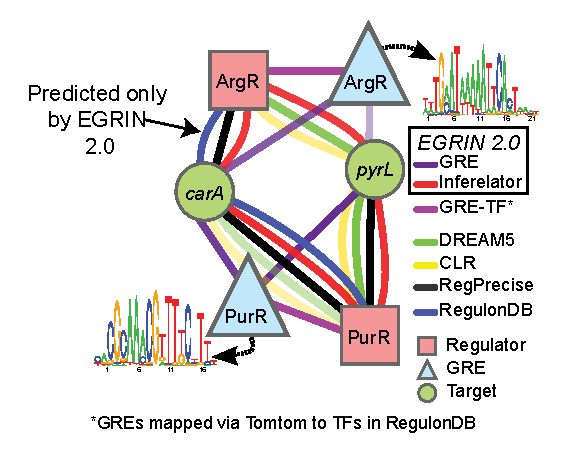
\includegraphics[width=0.5\linewidth]{figures/argR_purR_networks.pdf}
\caption[Integration of GRE discovery and \nwinf\ predictions
  yields comprehensive and detailed gene regulatory
  networks]{\textbf{Integration of GRE discovery and \nwinf\ 
    predictions yields comprehensive and detailed gene regulatory
    networks.} \egrine-inferred \textit{E. coli} regulatory subnetwork
  for two genes (green circles) in the PurR/ArgR regulon:
  \textit{carA} (\textit{b0032}) and \textit{pyrL} (\textit{b4246}).
  The \egrine~predictions are divided into GRE-based (dark violet) and
  \nwinf-based (red), and compared to predictions (or
  annotations) from other algorithms/databases (yellow: \tmsamp{CLR}; green:
  DREAM5 ensemble; black: \tmsamp{RegPrecise}; blue: \tmsamp{RegulonDB}). In two cases
  (ArgR$\rightarrow$carA and ArgR$\rightarrow$pyrL), \egrine~discovers
  regulatory interactions that were missed by either hand-curated
  databases or expression-based inference procedures.}
\label{fig:argR_purR_networks}
\end{figure} 

\subsection{Validation of condition-specific operon isoforms by tiling array transcriptome measurements}

We validated the prevalence of multiple, condition-specific
transcriptional isoforms from operons in \eco\ by measuring changes in
the transcriptome across growth, from lag-phase (OD600 = 0.05) to late
stationary phase (OD600 = 7.3). The experimental platform and other
experimental details are described in Section
\ref{section:ecoarray}. We used multivariate recursive partitioning,
including signals from both relative changes in expression along the
growth curve, as well as raw RNA hybridization signal to call putative
transcription breaks as previously described \cite{Koide2009}. To
determine the significance of our finding, we computed a $p$-value
describing the significance of the overlap between our predictions
(see Section \ref{section:condop}) and the experimental observations
using the cumulative hypergeometric distribution.

Figures \ref{fig:dpp_ecoli_expression}, \ref{fig:galE}, and
\ref{fig:ptsh} below depict several operons annotated with
condition-specific transcriptional isoforms. We have integrated GRE
elements discovered near break sites with the transcriptional
measurements.

\begin{figure}[hp]
\centering
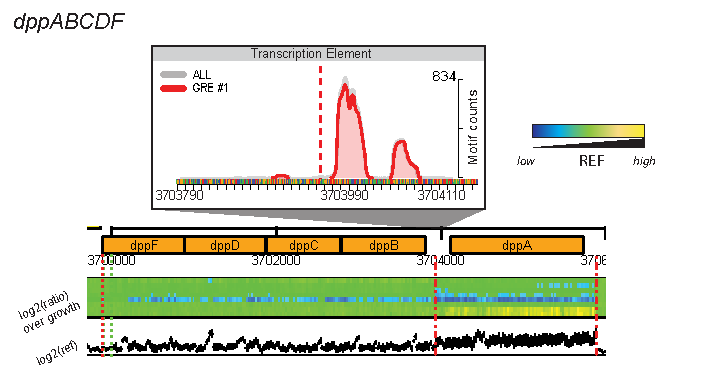
\includegraphics[width=0.7\linewidth]{figures/dpp_ecoli_expression.pdf}
\caption[GREs regulate multiple transcript isoforms from operons in
  {\it E. coli}, \textit{dppABCDF}]{\textbf{GREs regulate multiple
    transcript isoforms from operons in {\it E. coli},
    \textit{dppABCDF}.} GREs coincide with experimentally measured
  break sites. Three examples of experimentally determined
  transcription break sites (red dashed lines) in operons predicted by
  corems to be conditionally segmented. Expression levels of these
  regions were profiled across growth in rich media (heatmap). Inset
  contains region immediately surrounding a transcriptional break
  site, including counts of GREs discovered at these locations (as in
  Figure \ref{fig:nirH}).}
\label{fig:dpp_ecoli_expression}
\end{figure}

\begin{figure}[hp]
\centering
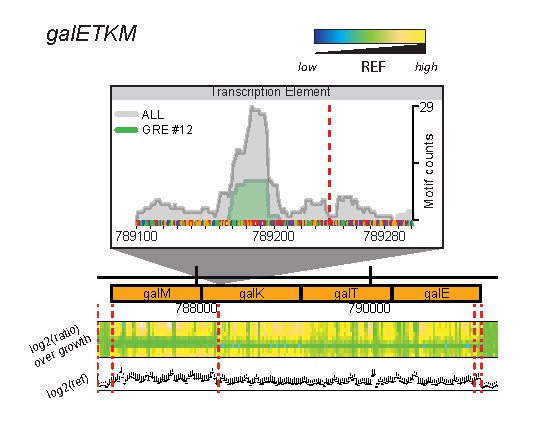
\includegraphics[width=0.7\linewidth]{figures/galE.pdf}
\caption[GREs regulate multiple transcript isoforms from operons in
  {\it E. coli}, \textit{galETKM}]{\textbf{GREs regulate multiple
    transcript isoforms from operons in {\it E. coli},
    \textit{galETKM}.} Caption details included in Figure
  \ref{fig:dpp_ecoli_expression}.}
\label{fig:galE}
\end{figure}

\begin{figure}[hp]
\centering
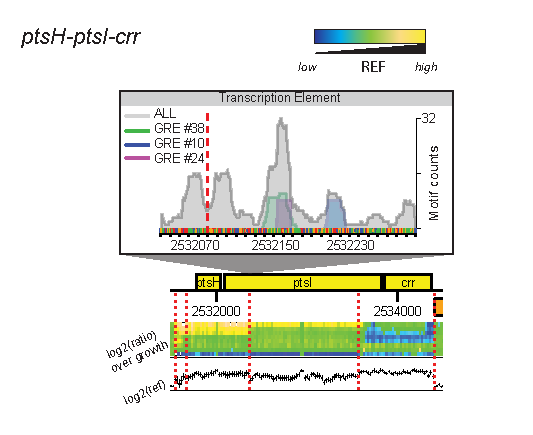
\includegraphics[width=0.7\linewidth]{figures/ptsh.pdf}
\caption[GREs regulate multiple transcript isoforms from operons in
  {\it E. coli}, \textit{ptsH-ptsI-crr}]{\textbf{GREs regulate
    multiple transcript isoforms from operons in {\it E. coli},
    \textit{ptsH-ptsI-crr}.} Caption details included in Figure
  \ref{fig:dpp_ecoli_expression}.}
\label{fig:ptsh}
\end{figure}

\subsection{Gene-gene co-fitness correlations in regulatory modules}

To assess the phenotypic consequences of co-regulation in corems, we
assessed whether genes grouped into corems had significantly similar
fitness consequences in many environments (\ie, the effect of deleting
one gene is highly similar to the effect of deleting the other across
many environments). We used the high-throughput fitness screen
described in Section \ref{section:fitness} to quantify these
relationships.

We compared the enrichment for high co-fitness relationships in corems
to other ways of assigning co-regulatory modules, including regulons
(\tmsamp{RegPrecise}, \rdb), operons, and \tmsamp{WGCNA}. The gene
modules for regulons (annotated in \rdb\ or \tmsamp{RegPrecise}
\cite{Novichkov2013}) consisted of genes annotated to a common TF. For
WGCNA, we assigned modules using the same community detection
procedures that we used to define corems from the \egrine~ensemble
(See \ref{section:gBg}). The gene co-expression modules were computed
from the weighted \tmsamp{WGCNA} adjacency matrix.

For the results presented in Figure~2B, we compared the distributions
of Pearson correlations between relative changes in fitness across
pairs of genes within each module, using the one-tailed
Kolmogorov-Smirnov test (KS-test). We report the KS $D$-statistic. The
precision/recall characteristics for each model are contained in Table~E5.

We extended this analysis by investigating whether the enriched high
co-fitness gene-gene relationships in corems consist of relationships
that could be described fully by regulons or operons. To answer this
question, we removed all gene pairs from corems that are also present
in operons or regulons and computed the KS-test again (Figure
\ref{fig:fitness_wo_operons}). We still observe a significant number
of high co-fitness relationships, suggesting that corems capture
physiologically meaningful co-regulatory relationships between genes
that cannot be explained by existing paradigms.

\begin{figure}[hp]
\centering
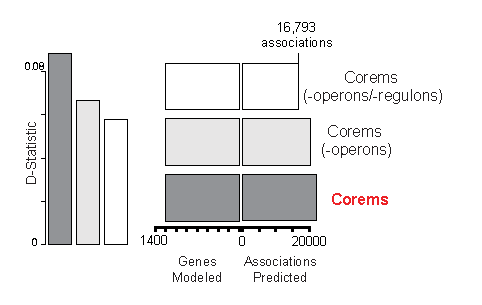
\includegraphics[width=0.6\linewidth]{figures/fitness_wo_operons.pdf}
\caption[\egrine~models highly correlated co-fitness relationships
  that cannot be explained by operons or
  regulons]{\textbf{\egrine~models highly correlated co-fitness
    relationships that cannot be explained by operons or regulons.}
  (Left) Enrichment for highly correlated, pairwise fitness
  measurements in gene knock outs across 324 conditions before and
  after removing gene associations annotated by operons
  (Microbes Online) and regulons (RegulonDB and RegPrecise)
  (KS-test,$D$-statistic). Two-thirds of gene-pairs with most highly
  correlated fitness within corems are not annotated by operons or
  regulons. (Right) Number of genes and associations predicted.}
\label{fig:fitness_wo_operons}
\end{figure}


\section{Model evaluation}\label{sec:evaluation}

In this section we evaluate the performance of the \egrine\ model as a function
of several important parameters. We focus in particular on how the
performance of the model changes as a function of the number of runs
included. From these evaluations, we conclude that (1) the model
performs well in its final form, (2) the model has reached a stable-state 
wherein inclusion of additional runs does not significantly increase model
performance, and (3) the model is not over-fit to particular
experiments within a data set or to any data set as a whole.

\subsection{Comparison with other module detection algorithms}

We compared the number of \rdb~TFs detected in the \egrine~model to individual
\cm~runs as well as to several other module detection/clustering
algorithms that were computed on subsets of the experimental data
(similar to the \egrine~ensemble; Figure \ref{fig:ensemble_comparison_regDB}). We
evaluated: (a) $k$-means clustering, (b) \tmsamp{WGCNA}
\cite{Langfelder2008}, and (c) \tmsamp{DISTILLER}
\cite{Lemmens2009}. For (a) and (b), we computed modules 100 times on
random subsets of the {\it E. coli} expression data set (using 200-250
randomly chosen experiments per run; selection criteria were identical
to {\it E. coli} \egrine; see Table~\ref{tab:cmparams:eco}). We then
predicted {\it de novo cis}-regulatory GREs in the promoter regions of genes
in each module using \tmsamp{MEME} (\tmsamp{MEME} parameters were also
identical to \egrine; Table~\ref{tab:cmparams:eco}). For (c), we
performed the comparison using the original modules generated by
\cite{Lemmens2009}. Rather than alter module composition by
re-detection, we instead varied \tmsamp{MEME} parameters applied to
the modules 100 times (again, within the same ranges as those used for
\egrine). TF-GRE matches were assigned by comparing GREs to
\rdb~TF binding sites, as previously described
(Section~\ref{section:tfbs:vs:regdb}).

We found that individual \cm~runs discovered a greater number of
\rdb~binding sites, on average, than the other methods (an average of
41 for \cm, compared to averages of 30, 25, and 29 for $k$-means,
\tmsamp{WGCNA}, and \tmsamp{DISTILLER}, respectively), which is
consistent with previous findings \cite{Reiss2006n}
(Figure~\ref{fig:ensemble_comparison_regDB}). Integration of all
\cm~biclusters into the complete \egrine~ensemble outperformed all
individual \cm~runs (53 total, as described in the Manuscript). This
result is typical of ensemble-based inference approaches, and supports
the value of ensemble integration as part of the \egrine\ model.

\begin{figure}[h!]
\centering
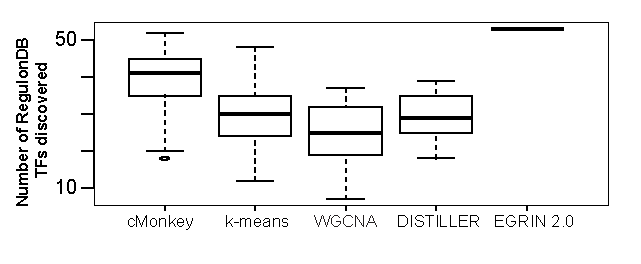
\includegraphics[width=0.6\linewidth]{figures/ensemble_comparison_regDB.pdf}
\caption[Number of TFs in \rdb~ re-discovered by various
    regulatory module detection methods.]  {{\bf Number of TFs in
    \rdb~ re-discovered by various regulatory module detection
    methods.} Comparison of \egrine~ (solid line, far right) to
  individual \cm\ runs, as well as multiple runs of $k$-means,
  \tmsamp{WGCNA}, and \tmsamp{DISTILLER} on subsets of the expression
  data. Evaluation made with respect to re-discovery of binding sites
  for 88 TFs with $\geq 3$ unique sites in \rdb~ based on genome-wide
  binding site locations (FDR $\leq 0.05$).}
\label{fig:ensemble_comparison_regDB}
\end{figure}

\subsection{Convergence and stability of the inferred network}

To evaluate the stability of the inferred \egrine\ network, we
quantified how the model changes as individual \cm\ runs are excluded
from the ensemble. Since the sub-bagging, as performed for
the \egrine\ model inference, %%(like cross-validation) is intended to
reduce model over-fitting, we used this evaluation understand whether
the model is over-fit to particular experiments in the data set. For
this task, we computed the number of individual EGRIN runs required to
converge on a consistent gene-gene co-occurrence network (see Section
\ref{section:gBg}). We computed gene-gene co-occurrence networks based upon randomly selected subsets of the 106 available \eco\ \cm\ runs, and varied the percentage selected between
1\%-99\% of the 106 runs. 5 replicate samples were computed for
each. To compare the networks, we computed the Pearson correlation
between the two matrices (sub-sampled gene-gene co-occurrence versus
the final \egrine\ gene-gene co-occurrence network). Note that since
the gene-gene co-occurrence network is a weighted adjacency matrix,
the correlation reflects the weighted discovery rate for every pair of
genes (rather than simple presence/absence). In
Figure \ref{fig:gBg_network_converge} we demonstrate that the
underlying networks converge rapidly to the final solution. By the
time $\sim 50$\% of the runs have been included ($\sim 50$ runs), the
inferred network is nearly identical to the final network ($\sim 100$
runs; cor $> 0.9$). The backbone extracted network takes a slightly
longer time to converge, likely because it requires more observations
of gene-gene pairs to retain them in the final network. Since corem
detection is deterministic and strictly based on the underlying
gene-gene co-occurrence matrix, this convergence means that the
inferred corems would be nearly identical even if up to half of the
runs were excluded.

\begin{figure}[h!]
\centering
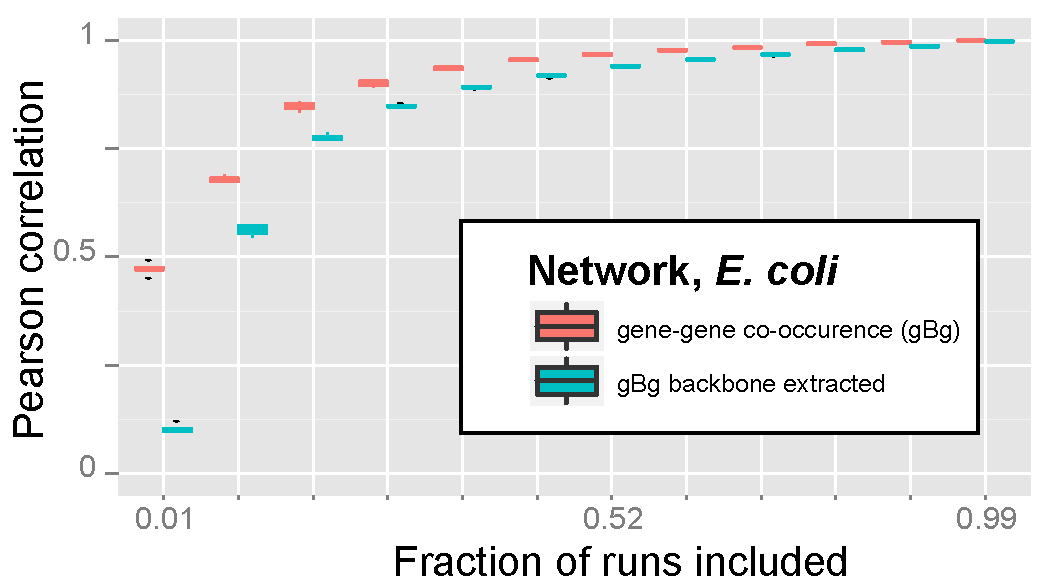
\includegraphics[width=0.75\linewidth]{figures/gBg_network_converge.pdf}
\caption[Convergence of \egrine\ gene co-occurrence networks.]  {
{\bf Convergence of \egrine\ co-occurrence networks.} The
co-regulation of genes predicted by the \eco\ \egrine\ model converges
rapidly to a stable network. Shown is the similarity of the gene-gene
co-occurrence matrix (and the backbone extraction of this matrix) to
the final \egrine\ \eco\ network, computed when varying fractions of
the \cm\ runs were excluded (Pearson correlation vs. the complete
model). Each point contains a box plot representing 5 replicate
sub-samples.}
\label{fig:gBg_network_converge}
\end{figure}

\subsection{Discovery of corems in an independent data set}

To determine whether \egrine\ model predictions are over-fit to
the \tmsamp{DISTILLER} expression compendium (or are the result of
biases in that data set), we tested whether support for corems existed
in an independent {\it E. coli} expression data set. Such evidence
would suggest that corems are \textit{bona fide} gene regulatory
modules that can be re-discovered in independent data, and that their
degree of condition-specificity is not biased due to normalization
differences in any given data set. For this test, we used
the \tmsamp{DREAM5} gene expression compendium. As described above
(Section \ref{section:dream5_data_compendium}), this data set is
comprised of different conditions, array platforms, and, most
important, was normalized by different methods, than
the \tmsamp{DISTILLER} data set used for model training. We determined
the condition-specific activity of corems in the \tmsamp{DREAM5} data
set using the methods described in Section \ref{section:rsd}. If a
corem was significantly co-expressed ($p$-value $\leq$ 0.05) in at
least one condition, we classified it `supported'. To our surprise, we
not only discovered support for $\sim 99$\% of the predicted corems,
we also discovered that their conditionality was very similar across
both data sets -- \ie, corems discovered to be co-expressed in few
conditions in the \tmsamp{DISTILLER} data set are also co-expressed in
few conditions in the \tmsamp{DREAM5} data set (same for corems
regulated in many conditions), and similarly for corems co-expressed
in a large number of conditions (Figure~\ref{fig:corem_conds_distiller_dream5}).
%% shows the number of conditions in which a corem is co-expressed across both data sets. 
Even after we removed the intrinsic relationship between the number of
genes in a corem and the number of conditions in which it is
co-expressed, we still observed a significant partial correlation of
0.49 ($p$-value $< 10^{-6}$) between the number of conditions in
corems as defined from the two data sets. 
%% The corems described in the main text({\color{red}ec512157}, {\color{blue}ec516034}, {\color{green}ec516031}) are indicated by their respective colors.

\begin{figure}[h!]
\centering
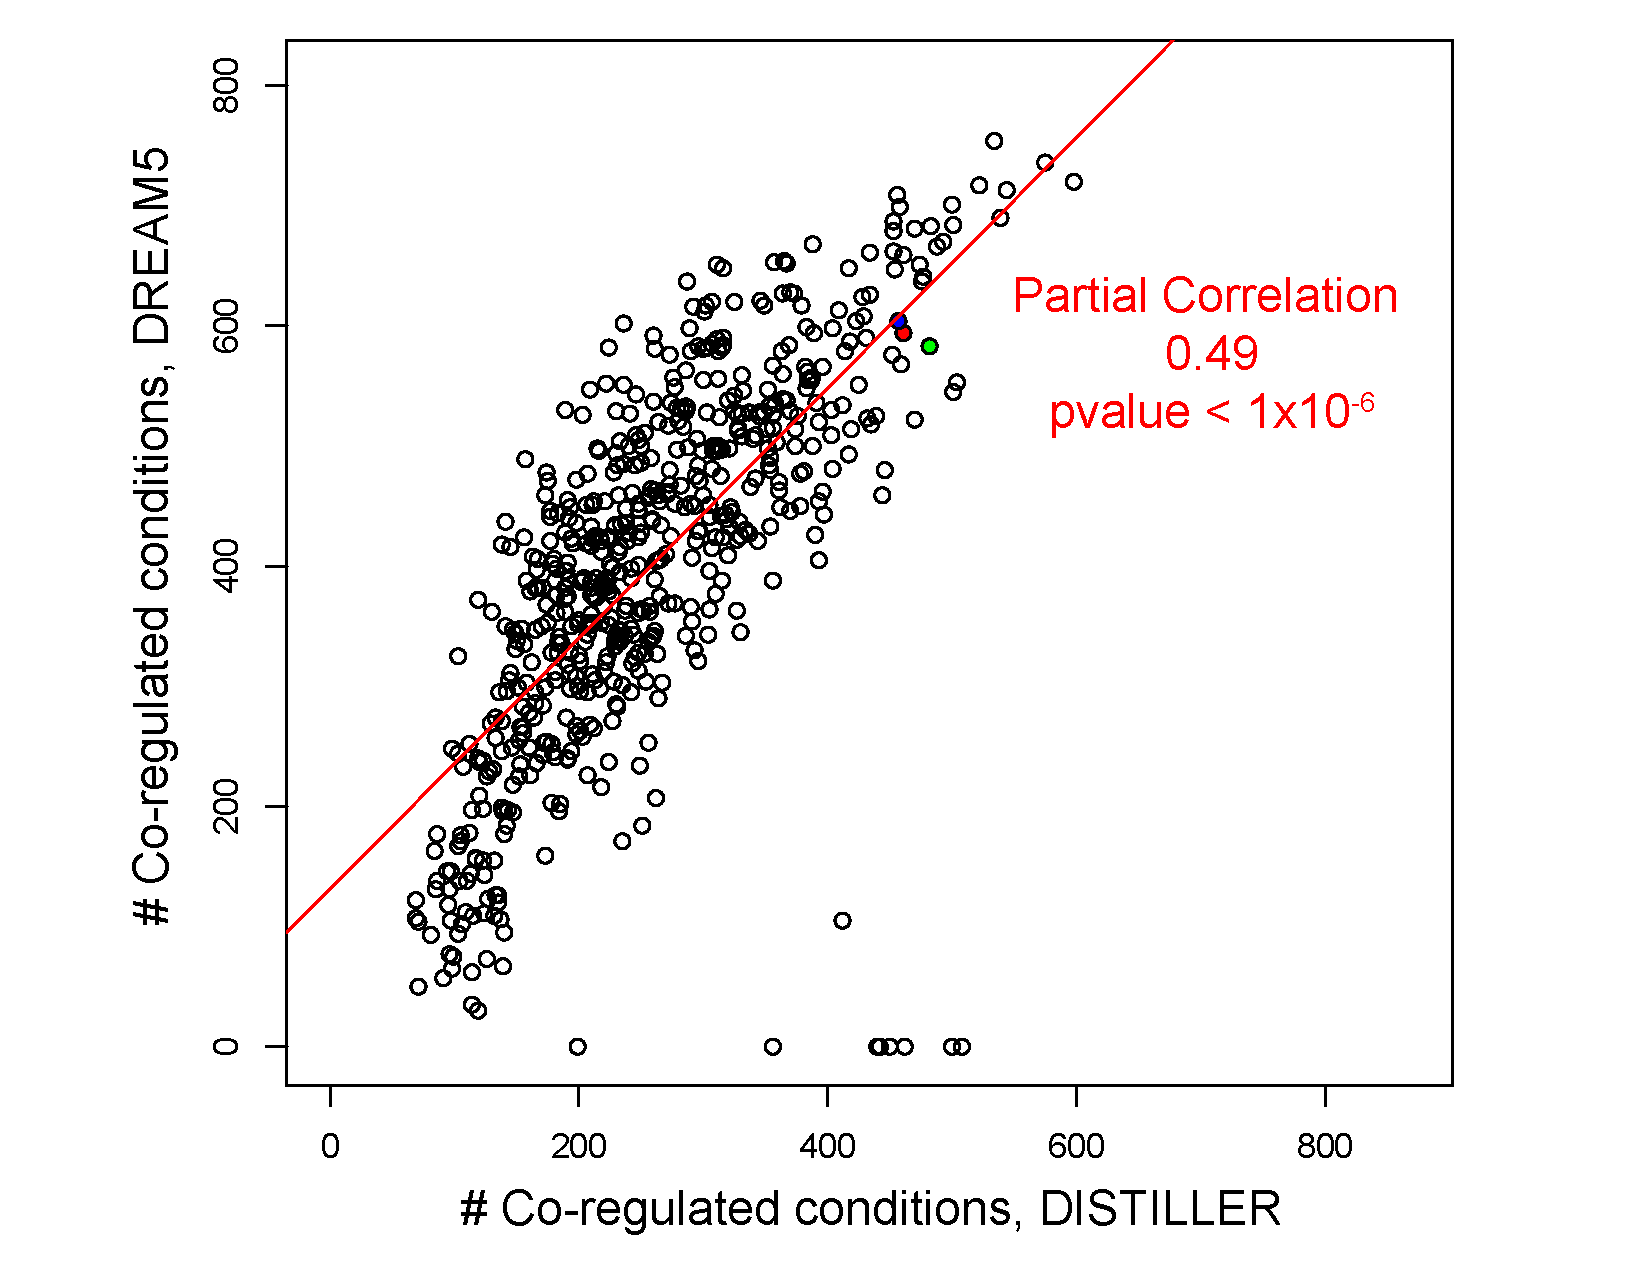
\includegraphics[width=0.6\linewidth]{figures/corem_conds_distiller_dream5.pdf}
\caption[Reproducibility of corems across data sets]{
\textbf{Reproducibility of corems across data sets.} 
Number of co-expressed conditions for corems in the \tmsamp{DISTILLER}
and \tmsamp{DREAM5} expression compendia. Conditions were selected as
in Section~\ref{section:rsd}. Significant partial correlation of 0.49
is observed after removing the affect of gene set size (log) on
the number of conditions co-expressed ($p$-value $< 10^{-6}$). The
three corems detailed in the main manuscript are identified with their
respective colors ({\color{red}ec512157}, {\color{blue}ec516034},
{\color{green}ec516031})}
\label{fig:corem_conds_distiller_dream5}
\end{figure}



\section{Additional Supporting Figures Referenced From Main Text}

\label{suppfigs}

\begin{figure}[hp]
\centering
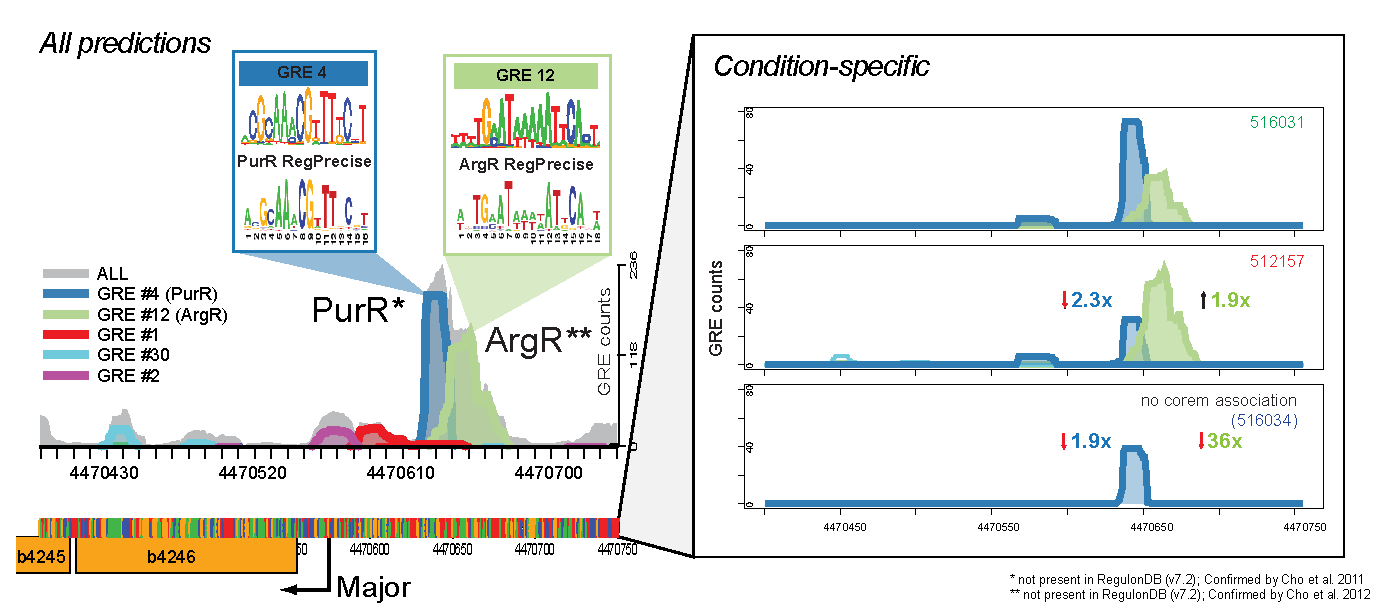
\includegraphics[width=0.95\linewidth]{figures/pyrL.pdf}
\caption[Differential GRE activity in \textit{pyrL} promoter, \textit{E. coli}]{\textbf{Differential GRE activity in \textit{pyrL} promoter, \textit{E. coli}.} (Left) Predicted promoter architecture for {\it E. coli} \textit{pyrL} (\textit{b4246}). Overlapping GREs matching to PurR (GRE \#4) and ArgR (GRE \#12) were detected upstream of pyrL. These sites were not annotated in RegulonDB, but were validated in independent ChIP-chip experiments \cite{Cho2012,Cho2011a}. Transcription start site indicated with arrow. (Bottom) Condition-specific promoter architectures for {\it E. coli} \textit{pyrL} (as in Figure 2E). Variation in predicted GRE activity across three different subsets of experimental conditions (counts and fold-change) for two GREs in the \textit{pyrL} promoter. Experimental subsets correspond to conditions under which at least one of three nucleotide biosynthetic corems is regulated (denoted by colored names at top-right of each plot)}
\label{fig:pyrL}
\end{figure}

\begin{figure}[hp]
\centering
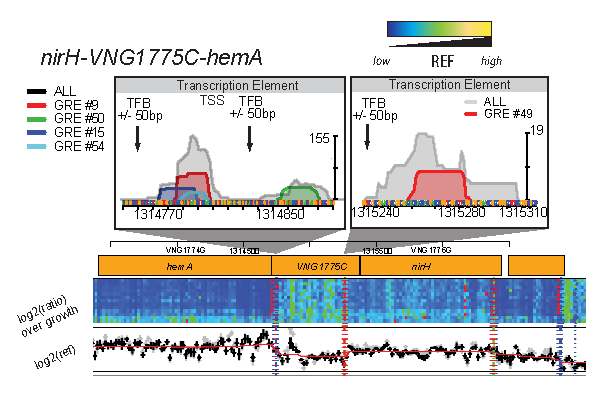
\includegraphics[width=0.95\linewidth]{figures/nirH.pdf}
\caption[GREs regulate multiple transcript isoforms from operons in {\it H. salinarum}, \textit{nirH-VNG1775C-hemA}.]{\textbf{GREs regulate multiple transcript isoforms from operons in {\it H. salinarum}, \textit{nirH-VNG1775C-hemA}.} GREs located inside operons coincide with experimentally measured transcriptional break sites. Experimentally determined transcription break sites (red dashed lines) above expression profiles of these regions across growth (heatmap, \cite{Koide2009} and ChIP-chip TFBs (\cite{Facciotti2007}, vertical arrows) support the role of GREs in regulating segmentation of the operon in certain conditions. Insets contain regions immediately surrounding transcriptional break sites, including counts of GREs discovered at these locations.}
\label{fig:nirH}
\end{figure}

\begin{figure}[hp]
\centering
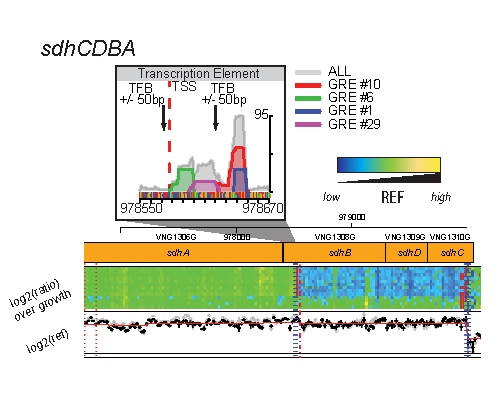
\includegraphics[width=0.95\linewidth]{figures/sdh.pdf}
\caption[GREs regulate multiple transcript isoforms from operons in {\it H. salinarum}, \textit{sdhCDBA}.]{\textbf{GREs regulate multiple transcript isoforms from operons in {\it H. salinarum}, \textit{sdhCDBA}.} Caption details included in Figure \ref{fig:nirH}}
\label{fig:sdh}
\end{figure}

\begin{figure}[hp]
\centering
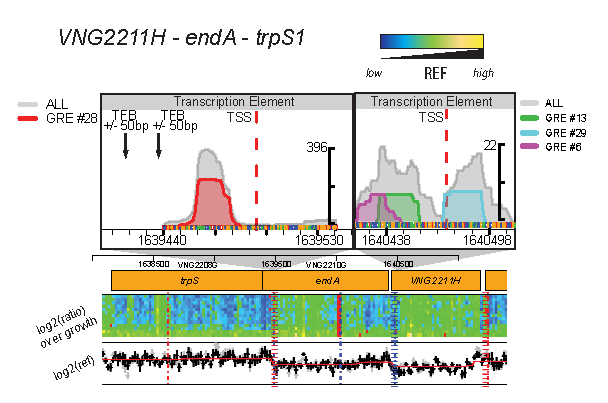
\includegraphics[width=0.95\linewidth]{figures/vng2211h.pdf}
\caption[GREs regulate multiple transcript isoforms from operons in {\it H. salinarum}, \textit{VNG2211H-endA-trpS1}.]{\textbf{GREs regulate multiple transcript isoforms from operons in {\it H. salinarum}, \textit{VNG2211H-endA-trpS1}.} Caption details included in Figure \ref{fig:nirH}}
\label{fig:vng2211h}
\end{figure}

\begin{figure}[hp]
\centering
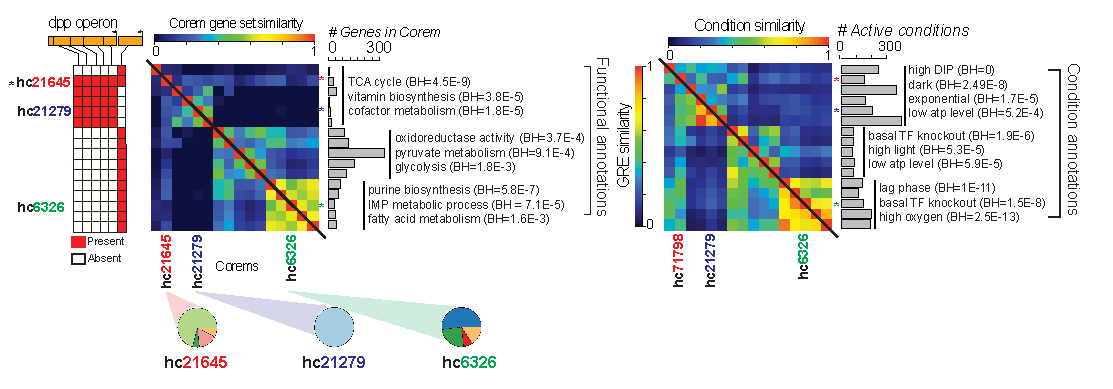
\includegraphics[width=0.95\linewidth]{figures/dpp_heatmaps.pdf}
\caption[Alternate regulatory modes for \textit{dpp} operon predicted by corems]{\textbf{Alternate regulatory modes for \textit{dpp} operon predicted by corems.} Corems group together functionally related sets of genes that are co-regulated in similar environments by similar factors (Left) Presence/absence of \textit{dpp} operon genes in corems. Three classes of corems exist for the dpp operon: (1) the entire operon (\eg hc21645), (2) the leader gene \textit{dppA} (\eg hc6326), and (3) five ``tail'' genes excluding \textit{dppA} (hc21279). (Middle) Gene similarity between corems (heatmap, Jaccard index). Functional annotations of genes in three highly similar clusters of corems to right. GRE composition for three corems shown below (pie chart, see Figure \ref{fig:corem_gres}). (Right) Similarity of conditions regulated (heatmap, upper triangle, Jaccard index) and GREs (heatmap, lower triangle, Jaccard index) among corems. Ordering is identical to (Middle). Environmental Ontology term enrichment (see ref{}) for three clusters depicted to right.}
\label{fig:dpp_heatmaps}
\end{figure}

\begin{figure}[hp]
\centering
\includegraphics[width=0.95\linewidth]{figures/dpp_networks.pdf}
\caption[Network representation of transcriptional isoforms for the \textit{dpp} operon predicted by corems]{\textbf{Network representation of transcriptional isoforms for the \textit{dpp} operon predicted by corems.} Network representation for three corems described in \ref{fig:dpp_heatmaps}. Genes represented by circles. Edge colors and colored region behind the network indicate corem membership. Pie charts reflect GRE composition of each gene (see Figure \ref{fig:corem_gres}). Key for pie charts at top. Shading behind nodes (center of network) indicates \textit{dpp} operon genes.}
\label{fig:dpp_networks}
\end{figure}

\begin{figure}[hp]
\centering
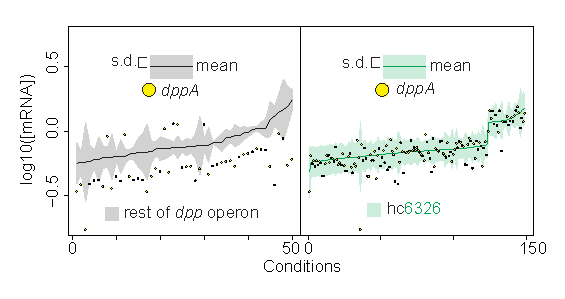
\includegraphics[width=0.95\linewidth]{figures/dpp_expression.pdf}
\caption[\textit{dppA} is more tightly co-expressed with genes of hc6326 in some environments than the other genes in the \textit{dpp} operon]{\textbf{\textit{dppA} is more tightly co-expressed with genes of hc6326 in some environments than the other genes in the \textit{dpp} operon.} Relative expression of \textit{dppA} compared to (left) other genes of \textit{dpp} opeon and (right) hc6326.}
\label{fig:dpp_expression}
\end{figure}

\begin{figure}[hp]
\centering
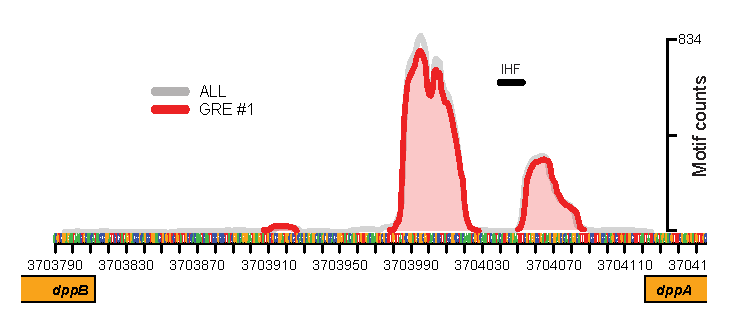
\includegraphics[width=0.95\linewidth]{figures/dpp_ecoli.pdf}
\caption[Evidence for condition-specific transcript isoforms of the \textit{dpp} operon in \textit{E. coli}]{\textbf{Evidence for condition-specific transcript isoforms of the \textit{dpp} operon in \textit{E. coli}.} \egrine~predicts conditional modulation of \textit{dpp} operon in {\it E. coli} as well. Promoter architecture within intergenic space between \textit{dppA} and \textit{dppB} suggested locations for TF binding internal to the operon (as in Figure 3A). GRE binding sites are proximal to an experimentally characterized IHF binding site (black horizontal bar; RegulonDB).}
\label{fig:dpp_ecoli}
\end{figure}

\begin{figure}[hp]
\centering
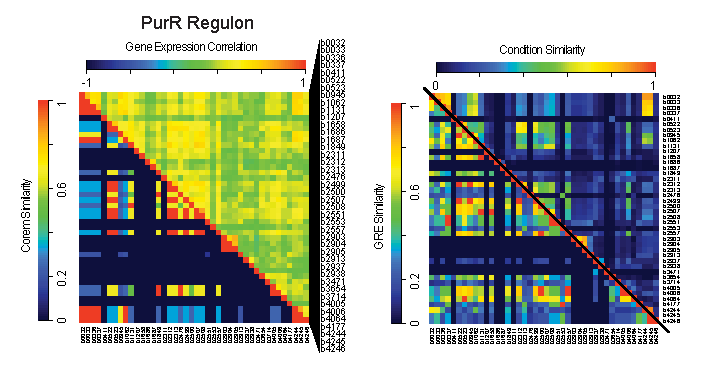
\includegraphics[width=0.95\linewidth]{figures/purR_heatmap.pdf}
\caption[Corems model the mechanistic basis for conditional subdivision of the PurR regulon, \textit{E. coli}]{\textbf{Corems model the mechanistic basis for conditional subdivision of the PurR regulon, \textit{E. coli}.} (Left) Corems identify the most highly correlated subgroupings of genes in PurR regulon. Gene expression correlation across all experiments (upper triangle) compared to similarity of corem membership (lower-triangle, Jaccard index) for genes of the PurR regulon (gene identifiers expanded to right). (Right) Similarity of regulated conditions (upper triangle, Jaccard index) and GREs composition for these genes (bottom triangle, Jaccard index). Consistent patterns of conditional-activity and GRE composition in their promoter regions further supports subdivision of PurR genes into separate corems. Gene order is same as left.}
\label{fig:purR_heatmap}
\end{figure}

\begin{figure}[hp]
\centering
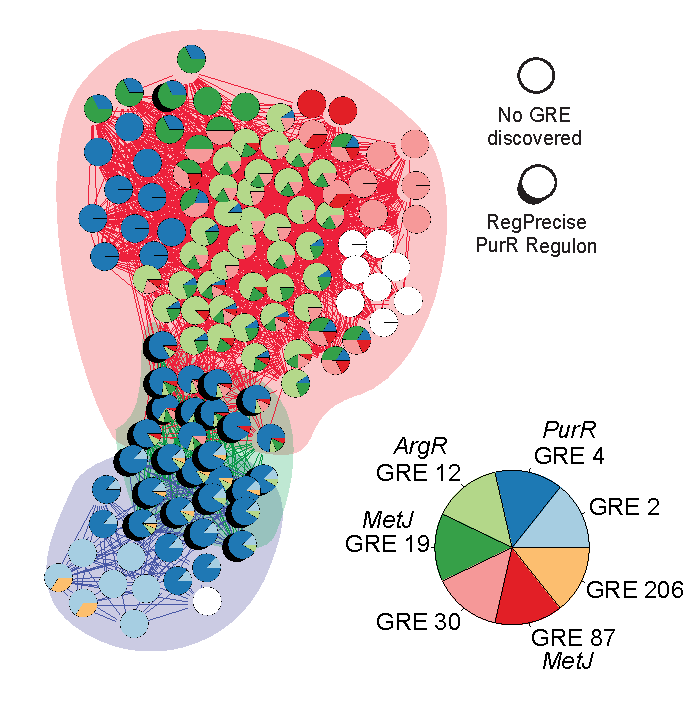
\includegraphics[width=0.95\linewidth]{figures/purR_network.pdf}
\caption[Corems integrate diverse regulatory mechanisms, \textit{E. coli}]{\textbf{Corems integrate diverse regulatory mechanisms, \textit{E. coli}.} Network representation for three corems described in Figure \ref{fig:purR_heatmap}. Genes are represented by circles. Edge colors and colored region behind the network indicate corem membership. Pie charts reflect GRE composition of each gene (see Figure~\ref{fig:corem_gres}). Key for pie charts at bottom. GRE-TF matches are indicated. Shading behind nodes denotes PurR regulon genes. At least 7 different mechanisms regulate the expression of these genes.}
\label{fig:purR_network}
\end{figure}


\begin{figure}[hp]
\centering
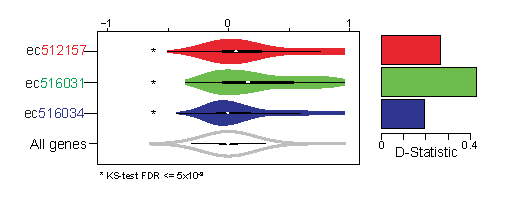
\includegraphics[width=0.95\linewidth]{figures/purR_corem_fitness.pdf}
\caption[Genes from corems related to nucleotide biosynthesis have highly similar fitness effects when they are deleted]{\textbf{Genes from corems related to nucleotide biosynthesis have highly similar fitness effects when they are deleted.} (Left) Violin plot shows distribution of all fitness correlations for genes in three nucleotide biosynthesis-associated corems compared to all genes in the data set. (Right) KS $D$-Statistic relates to enrichment for highly correlated gene-gene fitness associations in the corems. All three corems enrich for similar fitness effects (KS FDR $< 5\times 10^{-9}$)}
\label{fig:purR_corem_fitness}
\end{figure}

\begin{figure}[hp]
\centering
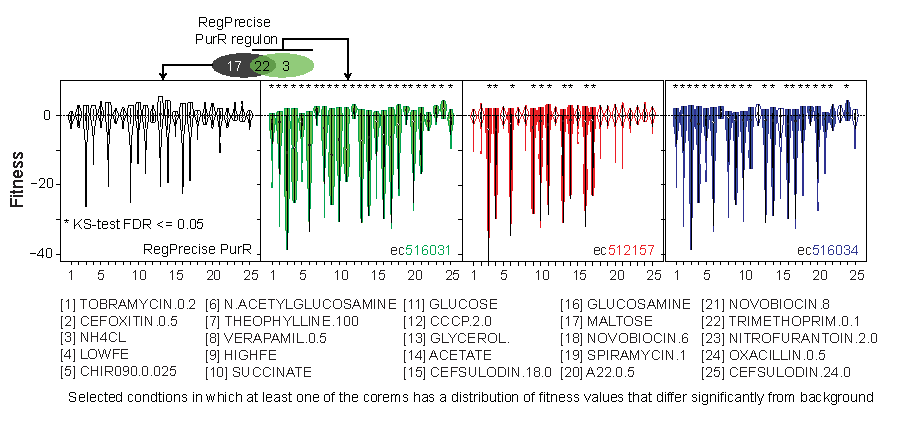
\includegraphics[width=0.95\linewidth]{figures/purR_corem_fitness_specific.pdf}
\caption[Corems model fitness effects that occur in specific environments]{\textbf{Corems model fitness effects that occur in specific environments.} Violin plots show distribution of relative fitness among corems across conditions (negative values indicate lower fitness relative to WT). Brief condition descriptions are displayed below. Shading within the violin plot indicates that the distribution of fitness values is significantly in that condition (KS-test FDR $\leq 0.05$). Fitness values for the subset of genes from the PurR regulon that do not occur in ec516031 are displayed to the left. These genes do not have significant fitness effects in any of the environments tested. Data from \cite{Nichols2011}.}
\label{fig:purR_corem_fitness_specific}
\end{figure}

\begin{figure}[hp]
\centering
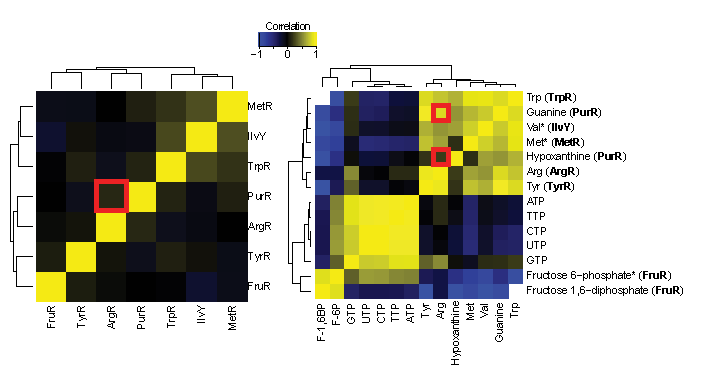
\includegraphics[width=0.95\linewidth]{figures/purR_effector.pdf}
\caption[Metabolite correlations may explain co-regulation within metabolically-linked corems]{\textbf{Metabolite correlations may explain co-regulation within metabolically-linked corems.} (Left) Expression correlation for TFs associated with three corems described in the text (ec516031,ec512157,ec516034). (Right) Correlation allosteric regulators for these TFs. TF regulated by each biomolecule listed in parentheses \cite{Novichkov2010}. Red boxes indicate PurR-ArgR and their corresponding effector molecules. Data from \cite{Ishii2007}.}
\label{fig:purR_effector}
\end{figure}

  %% slows it down and makes it big! Let's include it later.

\clearpage % force figures before bibliography
\bibliographystyle{abbrv}
\bibliography{egrin2_paper}{}

\end{document}
This is never printed
